\documentclass{report}

\def\class{report}
\def\lecorchap{Lecture}
\def\figloc{./figures/lec}
\def\noteloc{lectures/lec}

\setcounter{tocdepth}{2}

%%%%%%%%%%%%%%%%%%%%%%%%%%%%%%%%%%%%%%%%%%%%%%%%%%%%%%%%%%%%%%%%%%%%%%%%%%%%%%%%
%                                                                              %
%                              Required Packages                               %
%                                                                              %
%%%%%%%%%%%%%%%%%%%%%%%%%%%%%%%%%%%%%%%%%%%%%%%%%%%%%%%%%%%%%%%%%%%%%%%%%%%%%%%%

% Required for creating documents
\usepackage[utf8]{inputenc}
\usepackage[T1]{fontenc}
\RequirePackage{etex}

% Required math packages
\usepackage{amsmath}
\usepackage{amsfonts}
\usepackage{mathtools}
\usepackage{amsthm}
\usepackage{amssymb}
\usepackage{mathrsfs}

\usepackage{multicol} % for multiple columns
\usepackage[usenames,dvipsnames,pdftex]{color} % Required for nicer colors
\usepackage{hyperref} % Required for hyperlinks
\usepackage{xparse} % Required for \NewDocumentCommand
\usepackage{graphicx} % Required for including images
\usepackage{enumitem} % Required for customizing lists
\usepackage{float} % Required for positioning figures and tables
\usepackage{array} % Required for customizing tables
\usepackage{systeme} % Required for \systeme
\usepackage{cancel} % Required for \cancel
\usepackage{derivative} % Required for \odv and \pdv
\usepackage{authoraftertitle} % Required for \MyTitle
\usepackage{geometry} % Required for customizing page layout
\usepackage{textgreek} % Required for greek letters in text mode
\usepackage{multirow} % Required for multirow in tables
\usepackage{emptypage} % Required for removing page numbers on empty pages
\usepackage{nicematrix} % Required for better matrices
\usepackage{booktabs} % Required for better tables
\usepackage{cellspace} % Required for better spacing in tables
\usepackage{longtable} % Required for long tables
\usepackage{xfrac} % Required for extra fraction options
\usepackage{diagbox} % Required for creating diagonal boxes
\usepackage{polynom} % Required for polynomial long division
\usepackage{setspace} % For line spacing

\usepackage[font=bf]{caption} % Required for customizing captions
\usepackage{subcaption} % Required for creating subfigures
\usepackage{siunitx} % Required for SI units
\usepackage{titletoc} % Required for customizing table of contents
\usepackage{braket} % Required for creating braket notation

% Required for drawing figures
\usepackage{tikz}
\usepackage{pgffor}
\usepackage{tkz-euclide}
\usepackage{tikz-cd}
\usepackage{tikz-3dplot}
\usepackage{circuitikz}

% Required for creating plots
\usepackage{pgfplots}
\usepackage{pgfplotstable}

\usepackage{titling} % Required for customizing title page
\usepackage{ifthen} % Required for if-then-else statements
\usepackage{xifthen} % Required for if-then-else statements
\usepackage{fancyhdr} % Required for customizing headers and footers
\usepackage{import} % Required for importing pdf_tex files
\usepackage{titlesec} % Required for customizing sectioning commands
\usepackage{etex} % Required for more registers

% Required for creating boxes
\usepackage[most,many,breakable]{tcolorbox}

\makeatletter


%%%%%%%%%%%%%%%%%%%%%%%%%%%%%%%%%%%%%%%%%%%%%%%%%%%%%%%%%%%%%%%%%%%%%%%%%%%%%%%%
%                                                                              %
%                                Basic Settings                                %
%                                                                              %
%%%%%%%%%%%%%%%%%%%%%%%%%%%%%%%%%%%%%%%%%%%%%%%%%%%%%%%%%%%%%%%%%%%%%%%%%%%%%%%%

\ifx\nauthor\undefined
  \def\nauthor{Hashem A. Damrah}
\else
\fi

\ifx\class\undefined
  \def\class{report}
\else
\fi

\newcommand\globalcolor[1]{%
  \color{#1}\global\let\default@color\current@color
}

% Symbols
\let\oldlimsymbol\lim\renewcommand\lim{\displaystyle\oldlimsymbol}
\let\oldsumsymbol\sum\renewcommand\sum{\displaystyle\oldsumsymbol}
\let\oldlimsupsymbol\limsup\renewcommand\limsup{\displaystyle\oldlimsupsymbol}
\let\oldliminfsymbol\liminf\renewcommand\liminf{\displaystyle\oldliminfsymbol}
\let\implies\Rightarrow
\let\impliedby\Leftarrow
\let\iff\Leftrightarrow
\let\epsilon\varepsilon

% Geometry
\geometry{
  top=1in,
  bottom=1in,
  right=1in,
  left=1in,
}

% Tables
\newcolumntype{C}{>{\Centering\arraybackslash}X}
\setlength{\tabcolsep}{5pt}
\renewcommand\arraystretch{1.5}
\renewcommand\thetable{\Roman{table}}
\captionsetup[figure]{font=small}
\captionsetup{justification=centering}
\setlength\cellspacetoplimit{6pt}
\setlength\cellspacebottomlimit{6pt}

% Lists
\renewcommand{\labelitemi}{--}
\renewcommand{\labelitemii}{$\circ$}
\renewcommand{\labelenumi}{\textnormal{(\roman{*})}}

% Center Title Page
\let\@real@maketitle\maketitle
% \renewcommand\maketitle{
%   \@real@maketitle
%   \begin{center}
%     \begin{minipage}[c]{0.9\textwidth}
%       \centering\footnotesize
%       These notes are not endorsed by the lecturers, and
%       I have modified them (often significantly) after lectures. They are
%       nowhere near accurate representations of what was actually lectured, and
%       in particular, all errors are almost surely mine.

%       \textit{Disclaimer:} This document will inevitably contain some
%       mistakes--both simple typos and legitimate errors. Keep in mind that these
%       are the notes of an undergraduate student in the process of learning the
%       material himself, so take what you read with a grain of salt. If you find
%       mistakes and feel like telling me, I will be grateful and happy to hear
%       from you, even for the most trivial of errors. You can reach me by email,
%       in English, Arabic, Hebrew, or Spanish at
%       \href{mailto:singularisartt@gmail.com}{singularisartt@gmail.com}.
%     \end{minipage}
%   \end{center}
% }
\renewcommand\maketitlehooka{\null\mbox{}\vfill}
\renewcommand\maketitlehookd{\vfill\null}

% Footnote Line
\renewcommand\footnoterule{\hrule\vspace{0.1cm}}

% Modify Links Color
\hypersetup{
  colorlinks,
  linkcolor=black!90,
  citecolor=black,
  urlcolor=cyan!70!black,
}

%%%%%%%%%%
%  TikZ  %
%%%%%%%%%%

\usetikzlibrary{
  shadings,
  intersections,
  angles,
  quotes,
  calc,
  positioning,
  3d,
  perspective,
  arrows,
  arrows.meta,
  patterns,
  decorations.markings,
  bending,
  decorations.pathreplacing,
  calligraphy,
  backgrounds,
}

\tikzoption{canvas is xy plane at z}[]{%
	\def\tikz@plane@origin{\pgfpointxyz{0}{0}{#1}}%
	\def\tikz@plane@x{\pgfpointxyz{1}{0}{#1}}%
	\def\tikz@plane@y{\pgfpointxyz{0}{1}{#1}}%
	\tikz@canvas@is@plane}

\usetikzlibrary{shapes.arrows}
\newcommand\graphslopefield{
  \pgfmathsetmacro{\hx}{(\xmax-\xmin)/\nx}
  \pgfmathsetmacro{\hy}{(\ymax-\ymin)/\ny}
  \foreach \i in {0,...,\nx}
  \foreach \j in {0,...,\ny}{
    \pgfmathsetmacro{\yprime}{f({\xmin+\i*\hx},{\ymin+\j*\hy})}
    \draw[black,shift={({\xmin+\i*\hx},{\ymin+\j*\hy})}]
    (0,0)--($(0,0)!2mm!(.1,.1*\yprime)$);
  }

  \draw[->] (\xmin-.5,0)--(\xmax+.5,0) node[below right] {$x$};
  \draw[->] (0,\ymin-.5)--(0,\ymax+.5) node[above left] {$y$};
}

\tikzset{derivative/.style={color=gray,mark=none,line width=0.5pt,solid}}
\tikzset{asymptote/.style={color=gray,mark=none,line width=1pt,<->,dashed}}
\tikzset{soldot/.style={color=black,fill=black,only marks,mark=*}}
\tikzset{holdot/.style={color=black,fill=white,only marks,mark=*}}

\tikzset{>=stealth}
\tikzset{->-/.style={decoration={markings,mark=at position .5 with {\arrow{>}}},postaction={decorate}}}

%%%%%%%%%%%%%%
%  PgfPlots  %
%%%%%%%%%%%%%%

\pgfplotsset{width=7cm,compat=1.8}
\pgfplotsset{compat=newest}

\usepgfplotslibrary{patchplots}
\usepgfplotslibrary{fillbetween}
\usetikzlibrary{intersections}

\pgfplotsset{plot/.style={color=red,mark=none,line width=1pt,<->,solid}}
\pgfplotsset{asymptote/.style={color=gray,mark=none,line width=1pt,<->,dashed}}
\pgfplotsset{soldot/.style={color=red,only marks,mark=*}}
\pgfplotsset{holdot/.style={color=red,fill=white,only marks,mark=*}}
\pgfplotsset{blankgraph/.style={xmin=-10,xmax=10,ymin=-10,ymax=10,axis line style= {-, draw opacity=0 },axis lines=box,major tick length=0mm,xtick={-10,-9,...,10},ytick={-10,-9,...,10},grid=major,yticklabels={,,},xticklabels={,,},minor xtick=,minor ytick=,xlabel={},ylabel={},width=0.75\textwidth,grid style={solid,gray!40}}}

\pgfplotscreateplotcyclelist{stylelist}{
  plot \\
}

\def\axisdefaultwidth{175pt}
\def\axisdefaultheight{\axisdefaultwidth}

\pgfplotsset{every axis/.append style={
    axis x line=middle,
    axis y line=middle,
    axis line style={<->},
    xlabel={$x$},
    ylabel={$y$},
    xmin=-7,xmax=7,
    ymin=-7,ymax=7,
    yticklabel style={inner sep=0.333ex},
    minor xtick={-7,-6,...,7},
    minor ytick={-7,-6,...,7},
    scale only axis,
    cycle list name=stylelist,
    tick label style={font=\footnotesize},
    legend cell align=left,
    grid=minor,
    grid style={solid,gray!40},
    try min ticks=6,
  },
  framed/.style={axis background/.style={draw=gray}}
}

\pgfplotsset{axis background/.style={draw=gray}}


%%%%%%%%%%%%%%%%%%%%%%%%%%%%%%%%%%%%%%%%%%%%%%%%%%%%%%%%%%%%%%%%%%%%%%%%%%%%%%%%
%                                                                              %
%                           School Specific Commands                           %
%                                                                              %
%%%%%%%%%%%%%%%%%%%%%%%%%%%%%%%%%%%%%%%%%%%%%%%%%%%%%%%%%%%%%%%%%%%%%%%%%%%%%%%%

%%%%%%%%%%%%%%%%%%%%%%
%  Helpful Commands  %
%%%%%%%%%%%%%%%%%%%%%%

\newcommand\resetcounters{
  \setcounter{section}{0}
  \setcounter{subsection}{0}
  \setcounter{subsubsection}{0}
  \setcounter{paragraph}{0}
  \setcounter{subparagraph}{0}
}

\newcommand*\cleartoleftpage{%
  \clearpage
  \thispagestyle{empty}
  \ifodd\value{page}\else\hbox{}\newpage\fi
}

%%%%%%%%%%%%%%%%%%%%%%%%%%%%%
%  Lecture/Chapter Command  %
%%%%%%%%%%%%%%%%%%%%%%%%%%%%%

\def\notenum{}
\def\@note{}%
\newcommand\lecture[3]{
  \ifthenelse{\isempty{#3}}{%
    \def\@note{Lecture #1}%
  }{%
    \def\@note{Lecture #1: #3}%
  }%
  \section*{\@note\hfill{\small\textnormal{#2}}}
}

% Intro
\newcommand\createintro{
  \maketitle

  \pagenumbering{roman}
  \begin{center}
    \textbf{{\LARGE Introduction}}
    \phantomsection\addcontentsline{toc}{chapter}{0\hspace{0.8em}Introduction}
  \end{center}

  \begingroup
  \IfFileExists{./intro.tex}{
    \setlength{\parindent}{1cm}
    Lecture notes from the course \MyTitle, given by professor Victor Ostrik at the \faculty~at \location~in the academic year \academicyear, during the \term term. This course covers symbolic logic, basic set theory, analyzing functions and their properties, modular arithmetic, counting and other problems in discrete mathematics, induction, and convergence of sequences and continuity of functions. Credit for the material in these notes is due to professor Victor, while the structure is loosely taken from the \href{https://www.amazon.com/Mathematical-Reasoning-Writing-Proof-2nd/dp/0131877186}{Mathematical Reasoning: Writing and Proof} textbook. The credit for the typesetting is my own.

\textit{Disclaimer:} This document will inevitably contain some mistakes--both simple typos and legitimate errors. Keep in mind that these are the notes of an undergraduate student in the process of learning the material himself, so take what you read with a grain of salt. If you find mistakes and feel like telling me, I will be grateful and happy to hear from you, even for the most trivial of errors. You can reach me by email, in English, Arabic, Hebrew, or Spanish at \href{mailto:singularisartt@gmail.com}{singularisartt@gmail.com}.

  }{}
  \endgroup

  \pagestyle{fancy}
  \renewcommand\headrulewidth{0pt}

  \fancyhead{}
  \fancyfoot[C]{%
    \textit{For more notes like this, visit \href{\linktootherpages}{\shortlinkname}}.%
  }%

  \begin{tcolorbox}[
      enhanced,
      colback=white,
      center upper,
      size=fbox,
      drop shadow southwest,
      sharp corners,
    ]
    \term: \academicyear, \\
    Last Update: \today, \\
    \faculty, \location.
  \end{tcolorbox}

  \newpage
  \tableofcontents

  \pagenumbering{arabic}
  \setcounter{page}{1}

  \renewcommand\headrulewidth{0.4pt}
  \fancyhead[R]{\@note}
  \fancyhead[L]{\nauthor}
  \fancyfoot[C]{\thepage}
}

%%%%%%%%%%%%%%%%%%%%%
%  Random Commands  %
%%%%%%%%%%%%%%%%%%%%%

% Circle
\newcommand*\circled[1]{
  \tikz[baseline=(char.base)] {
    \node[shape=circle,draw,inner sep=1pt] (char) {#1};
  }
}

% Import Figures
\newcommand\incimg[2][1]{%
  \includegraphics[width=#1\columnwidth]{figures/#2}%
}

\newcommand\incfig[2][1]{
  \def\svgwidth{#1\columnwidth}
  \import{figures}{#2.pdf_tex}
}

% Correct
\newcommand\correct[1]{\textcolor{correct}{#1}}
\newcommand\incorrect[1]{{\color{incorrect}#1}}
\newcommand\inctocor[2]{\incorrect{#1} \ensuremath{\to} \correct{#2}}

% Bracket
\renewcommand\bra[1]{\left\langle#1\right|}
\renewcommand\ket[1]{\left|#1\right\rangle}
\renewcommand\braket[2]{\left\langle#1\middle|#2\right\rangle}
\renewcommand\ang[1]{\left\langle#1\right\rangle}

% For diagonal strikeout in red
\newcommand\rcancel[1]{\renewcommand\CancelColor{\color{red}}\cancel{#1}}

% Logic
\renewcommand\nmid{\not|~}

% For differentials
\newcommand\dd[1]{\textrm{d}#1}
\newcommand\dA{\textrm{d}A}
\newcommand\dm{\textrm{d}m}
\newcommand\dt{\textrm{d}t}
\newcommand\dT{\textrm{d}T}
\newcommand\du{\textrm{d}u}
\newcommand\dv{\textrm{d}v}
\newcommand\dx{\textrm{d}x}
\newcommand\dy{\textrm{d}y}
\newcommand\dz{\textrm{d}z}

% Helpful text in math
\newcommand\abs{\text{abs}}
\newcommand\echelon{\underrightarrow{\textrm{ echelon form }}}
\newcommand\rref{\underrightarrow{\textrm{ rref }}}
\newcommand\pick[1]{\xrightarrow[#1]{\textrm{ pick }}}
\newcommand\generalsol{\xrightarrow[\textrm{solution}]{\textrm{ general }}}
\newcommand\ngeneralsol{\parbox{4em}{general \\ solution}\textrm{:}}
\renewcommand\and{\text{and}}
\newcommand\aand{\quad\text{and}\quad}
\newcommand\adj{\text{adj}}
\newcommand\qtq[1]{\quad\textrm{#1}\quad}
\newcommand\oor{\quad\text{or}\quad}
\newcommand\Col{\textrm{Col}}
\newcommand\Nul{\textrm{Null}}
\newcommand\range{\textrm{Range}}
\newcommand\Tr{\textrm{Tr}}
\newcommand\Row{\textrm{Row}}
\newcommand\rank{\textrm{rank}}
\newcommand\dist{\text{dist}}
\newcommand\sz{\stackrel{\textrm{set}}{=}}
\newcommand\ce{\overset{\checkmark}{=}}
\newcommand\proj{\text{proj}}
\newcommand\comp{\text{comp}}
\newcommand\Card{\text{Card}}
\renewcommand\mod{\text{mod}}
\newcommand\st{\text{such that}}
\newcommand\geogebra{\textsf{GeoGebra}}
\newcommand\Sspan{\text{Span}}
\renewcommand\Re{\text{Re}}
\renewcommand\Im{\text{Im}}

% Laplace
\newcommand\laplace[1]{\mathscr{L}\left\{#1\right\}}
\newcommand\ilaplace[1]{\mathscr{L}^{-1}\left\{#1\right\}}

% Vectors
\renewcommand\a{\mathbf{a}}
\renewcommand\b{\mathbf{b}}
\renewcommand\c{\mathbf{c}}
\renewcommand\d{\mathbf{d}}
\newcommand\e{\mathbf{e}}
\newcommand\f{\mathbf{f}}
\newcommand\g{\mathbf{g}}
\newcommand\n{\mathbf{n}}
\newcommand\p{\mathbf{p}}

\newcommand\RR{\mathbf{R}}
\newcommand\FF{\mathbf{F}}

\renewcommand\r{\mathbf{r}}
\newcommand\rr{\mathbf{r}^{\prime}}
\newcommand\rrr{\mathbf{r}^{\prime\prime}}

\newcommand\Ta{\mathbf{T}}
\newcommand\Taa{\mathbf{T}^{}}

\renewcommand\u{\mathbf{u}}
\newcommand\uu{\mathbf{u}^{\prime}}
\newcommand\uuu{\mathbf{u}^{\prime\prime}}

\renewcommand\v{\mathbf{v}}
\newcommand\vv{\mathbf{v}^{\prime}}
\newcommand\vvv{\mathbf{v}^{\prime\prime}}

\newcommand\w{\mathbf{w}}
\newcommand\x{\mathbf{x}}
\newcommand\y{\mathbf{y}}
\newcommand\z{\mathbf{z}}

\newcommand\zero{\mathbf{0}}

% Hat vectors
\newcommand\ah{\hat{\mathbf{a}}}
\newcommand\bh{\hat{\mathbf{b}}}
\newcommand\ch{\hat{\mathbf{c}}}
\renewcommand\dh{\hat{\mathbf{d}}}
\newcommand\eh{\hat{\mathbf{e}}}
\newcommand\ph{\hat{\mathbf{p}}}
\newcommand\uh{\hat{\mathbf{u}}}
\newcommand\vh{\hat{\mathbf{v}}}
\newcommand\wh{\hat{\mathbf{w}}}
\newcommand\xh{\hat{\mathbf{x}}}
\newcommand\yh{\hat{\mathbf{y}}}
\newcommand\zh{\hat{\mathbf{z}}}

% Unit vectors
\newcommand\ui{\mathbf{i}}
\newcommand\uj{\mathbf{j}}
\newcommand\uk{\mathbf{k}}

% Subspaces
\newcommand\B{\mathcal{B}}
\newcommand\CC{\mathbb{C}}
\newcommand\C{\mathcal{C}}
\newcommand\D{\mathcal{D}}
\newcommand\E{\mathcal{E}}
\newcommand\F{\mathcal{F}}
\newcommand\I{\mathbb{I}}
\newcommand\N{\mathbb{N}}
\newcommand\Q{\mathbb{Q}}
\newcommand\R{\mathbb{R}}
\newcommand\U{\mathcal{U}}
\newcommand\W{\mathbf{w}}
\newcommand\X{\mathcal{X}}
\newcommand\Y{\mathcal{Y}}
\newcommand\Z{\mathbb{Z}}

% Create command to box equations
\newcommand*\colorboxed{}
\def\colorboxed#1#{%
  \colorboxedAux{#1}%
}
\newcommand*\colorboxedAux[3]{%
  \begingroup
    \colorlet{cb@saved}{.}%
    \color#1{#2}%
    \boxed{%
      \color{cb@saved}%
      #3%
    }%
  \endgroup
}
\newcommand\empheq[1]{%
  \colorboxed{black}{%
    \begin{aligned}[b]
      #1
    \end{aligned}%
  }%
}


%%%%%%%%%%%%%%%%%%%%%%%%%%%%%%%%%%%%%%%%%%%%%%%%%%%%%%%%%%%%%%%%%%%%%%%%%%%%%%%%
%                                                                              %
%                                 Environments                                 %
%                                                                              %
%%%%%%%%%%%%%%%%%%%%%%%%%%%%%%%%%%%%%%%%%%%%%%%%%%%%%%%%%%%%%%%%%%%%%%%%%%%%%%%%

\theoremstyle{definition}
\newtheorem*{assumption}{Assumption}
\newtheorem*{claim}{Claim}
\newtheorem*{conjecture}{Conjecture}
\newtheorem*{definition}{Definition}
\newtheorem*{example}{Example}
\newtheorem*{notation}{Notation}
\newtheorem*{proposition}{Proposition}
\newtheorem*{question}{Question}
\newtheorem*{problem}{Problem}
\newtheorem*{rrule}{Rule}

\newtheorem*{remark}{Remark}
\newtheorem*{note}{Note}
\newtheorem*{warning}{Warning}

\theoremstyle{plain}
\newtheorem*{corollary}{Corollary}
\newtheorem*{lemma}{Lemma}
\newtheorem*{theorem}{Theorem}
\newtheorem*{worksheet}{Worksheet}

\newcommand\frmebox[1][]{%
  \begin{tcolorbox}[%
    title={\sffamily\color{black}#1},
    colback=white,
    enhanced,
    attach boxed title to top center={
      yshift=-3mm,
      yshifttext=-1mm,
    },
    boxed title style={
      size=small,
      colback=white,
      frame code={},
    },
    coltext=black,
    frame hidden,
    borderline east={0.5pt}{0pt}{black},
    borderline west={0.5pt}{0pt}{black},
    borderline north={0.5pt}{0pt}{black},
    borderline south={0.5pt}{0pt}{black},
    breakable,
    parskip=0pt,
  ]
}

\renewenvironment{frame}[1][]{%
  \frmebox[#1]%
}{%
  \end{tcolorbox}%
}

\makeatother


\title{Fundamentals of Analysis I}
\author{Hashem A. Damrah}
\date{September 30, 2024}

\newcommand\linktootherpages{https://singularisart.github.io/notes}
\newcommand\shortlinkname{singularisart.github.io/notes}
\newcommand\term{Fall}
\newcommand\academicyear{$2024$}
\newcommand\faculty{Faculty of Mathematics}
\newcommand\location{University of Oregon}

\begin{document}
  \createintro
  \newpage

  \chapter{The Real Numbers}
  \label{chap:the_real_numbers}

  % notes start 1-5
  \nte{Sep 30 2024 Mon (13:01:47)}{TEMP}



\newpage

  \lecture{2}{Oct 2 2024 Wed (13:02:51)}{Triangle Inequality}

\section{Functions}

\begin{definition}[Function]
  Let $A$ and $B$ be two sets. A \emph{function} $f : A \to B$ assigns an
  element from the \emph{domain} $A$ to the \emph{range} $B$.
\end{definition}

\begin{example}
  Let $A$ be the set of chairs in a classroom and let $B$ be the set of all
  students in the room. Then, $f : A \to B$ assigns each chair to a student,
  like a seating chart.
\end{example}\leavevmode\vspace{-0.8cm}

\begin{example}
  Let $f(x) = x^2 + 1$, where $f : \R \to \R$. Then, the domain of $f$ is $\R$
  and the range is the interval $[1, \infty)$.
\end{example}

% section functions (end)

\section{Triangle Inequality}

The absolute value function is so important, that it has it's own notation,
$\lvert x \rvert$ in place of the usual $f(x)$. It's defined as
\begin{equation}
  \empheq{
    \lvert x \rvert = \begin{cases}
      x & \text{if}~x \geq 0, \\
      -x & \text{if}~x < 0
    \end{cases}
  }
\end{equation}

The absolute value function satisfies the following properties
\begin{enumerate}
  \item $\lvert ab \rvert = \lvert a \rvert \cdot \lvert b \rvert$.

  \item $\lvert a + b \rvert \le \lvert a \rvert + \lvert b \rvert$.
\end{enumerate}

The second property is known as the \emph{Triangle Inequality}, and it's mostly
used with three numbers, $a$, $b$, and $c$. Rearranging the inequality, we get
\[%
  \lvert a - b \rvert = \lvert (a - c) + (c - b) \rvert \implies \lvert (a - c) + (c - b) \rvert \le \lvert a - c \rvert + \lvert c - b \rvert
,\]%
giving us
\begin{equation}\label{eq:triangle_inequality}
  \empheq{\lvert a - b \rvert \le \lvert a - c \rvert + \lvert c - b \rvert}
\end{equation}

\begin{note}
  The expression $\lvert a - b \rvert$ is the distance between $a$ and $b$ on
  the real number line, which is also equivalent to $\lvert b - a \rvert$.
\end{note}

Restating the triangle inequality in terms of distance, we get that the distance
between $a$ and $b$ is less than or equal to the sum of the distances between
$a$ and $c$ and $c$ and $b$.

% section triangle_inequality (end)

  \lecture{3}{Oct 4 2024 Fri (13:00:10)}{Axiom of Completeness}

The defining difference between $\R$ and $\Q$ is that $\R$ does not contain the gaps that permeate $\Q$. We will be precise about how we phrase this assumption. This is referred to as the \emph{Axiom of Completeness}.
\begin{frame}[Axiom of Completeness]
  \begin{center}
    Every nonempty set of real numbers that is bounded above has a least upper bound.
  \end{center}
\end{frame}

\begin{note}
  We will never be able to prove the Axiom of Completeness, as axioms are meant to be taken as true. However, this will be the only statement that we naively accept without any rigorous proof. Everything else will be proven from this axiom.
\end{note}

Now, let's break down the definition of the least upper bound.

\subsection{Least Upper Bound and Greatest Lower Bound}

\begin{definition}[Upper Bound]
  A set $A \subseteq \R$ is bounded above if $(\exists b \in \R)(\forall a \in A)[a \le b]$. The number $b$ is called the \emph{upper bound} for $A$.
\end{definition}

\begin{definition}[Least Upper Bound]
  A real number $s$ is the \emph{least upper bound} for a set $A \subseteq \R$ if it meets the following two criteria
  \begin{enumerate}
    \item $s$ is an upper bound for $A$.

    \item If $b$ is any upper bound for $A$, then $s \le b$.
  \end{enumerate}
\end{definition}

\begin{example}
  Take the set $A = [-M, M]$. Then, all the numbers $m \ge M$ are upper bounds for $A$, while, only $M$ is the least upper bound.
\end{example}

The least upper bound is also called the \emph{supremum} of the set $A$. The \emph{greatest lower bound}/\emph{infimum} for $A$ is also defined similarly (see the figure below for a graphical representation).
\begin{figure}[H]
  \centering

  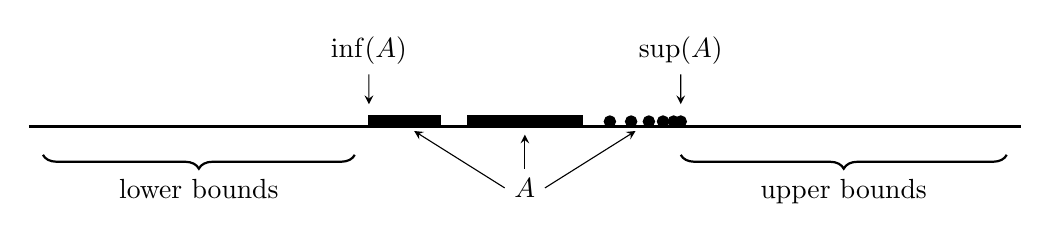
\begin{tikzpicture}[scale=0.9]
    \draw[thick] (-7, 0) -- (7, 0);

    % lower bounds from -6.8 to -2.4
    \draw[decorate,decoration={mirror,brace,amplitude=5pt},thick] (-6.8, -0.4) -- (-2.4, -0.4) node[midway, below=5pt] {lower bounds};

    % The set A from -2.2 to 2.2
    \draw[thick,fill=black] (-2.2, 0) -- (-2.2, 0.15) -- (-1.2, 0.15) -- (-1.2, 0) -- cycle;
    \node[above=15pt] (Inf) at (-2.2,0.15) {$\inf(A)$};
    \node[above=1pt] (Box1) at (-2.2,0) {};
    \draw[arrows={->}] (Inf) edge (Box1);

    \draw[thick,fill=black] (-0.8, 0) -- (-0.8, 0.15) -- (0.8, 0.15) -- (0.8, 0) -- cycle;

    \draw[soldot] (2.2,0.07) circle (0.08);
    \draw[soldot] (2.1,0.07) circle (0.08);
    \draw[soldot] (1.95,0.07) circle (0.08);
    \draw[soldot] (1.75,0.07) circle (0.08);
    \draw[soldot] (1.5,0.07) circle (0.08);
    \draw[soldot] (1.2,0.07) circle (0.08);

    \node[above=15pt] (Sup) at (2.2,0.15) {$\sup(A)$};
    \node[above=1pt] (Box2) at (2.2,0) {};
    \draw [arrows={->}] (Sup) edge (Box2);

    \node[below=5pt] (A) at (0,-0.4) {$A$};
    \node[below=1pt] (O) at (0,0.2) {};
    \draw[arrows={->}] (A) edge (O);

    \node[below=1pt] (AE1) at (-1.7,0.2) {};
    \draw[->] (A.west) -- (AE1);

    \node[below=1pt] (AE2) at (1.7,0.2) {};
    \draw[->] (A.east) -- (AE2);

    % upper bounds from 2.2 to 6.8
    \draw[decorate,decoration={mirror,brace,amplitude=5pt},thick] (2.2, -0.4) -- (6.8, -0.4) node[midway, below=5pt] {upper bounds};
  \end{tikzpicture}
\end{figure}

\begin{notation}
  The supremum is denoted as $s = \sup(A)$ and the infimum is denoted as $s = \inf(A)$.
\end{notation}

\begin{claim}
  A set that's bounded can only have one least upper bound.
\end{claim}

\begin{proof}
  By property (ii) of the definition of the least upper bound, if $s$ and $t$ are both least upper bounds for $A$, then $s \le t$ and $t \le s$, implying that $s = t$.
\end{proof}

\begin{example}
  The closed interval $[a, b]$ has a supremum of $b$ and an infimum of $a$. So does the open interval $(a, b)$. But what's the difference between the two? We'll investigate that later on.
\end{example}

\begin{example}
  Let $A = \left.\left\{\frac{1}{n}~\right\rvert n \in \N\right\} = \left\{1, \frac{1}{2}, \frac{1}{3}, \dots\right\}$. It's clear that $\sup(A) = 1$ and $\inf(A) = 0$.
\end{example}

\subsection{Maximum and Minimum}

\begin{definition}[Maximum and Minimum]
  A real number $a_0$ is a \emph{maximum} of the set $A$ if $a_0$ is an element of $A$ and $(\forall a \in A)[a_0 \ge a]$. Similarly, $a_0$ is a \emph{minimum} of the set $A$ if $a_0$ is an element of $A$ and $(\forall a \in A)[a_0 \le a]$.
\end{definition}

The closed interval $[a, b]$ has a maximum of $b$ and a minimum of $a$, since they're both elements of the set. However, the open interval $(a, b)$ has neither a maximum nor a minimum, since $a$ and $b$ aren't in the set.

\begin{example}
  Let $A = \left.\left\{1 + \frac{1}{n}~\right\rvert n \in \N\right\}$, giving us $\sup(A) = 2 = \max(A)$, but $\inf(A) = 1 \ne \min(A)$, as it does not exist.
\end{example}

\begin{question}
  Let $A \subseteq \R$ be nonempty and bounded above, let $c \in \R$. Define the set $c + A = \left\{c + a \mid a \in A\right\}$. Then, $\sup(c + A) = c + \sup(A)$.
\end{question}

\begin{proof}[Solution]
  Let $s = \sup(A)$. Let $a \in A$. Since $s$ is an upper bound of $A$, then $a \le s \implies a + c \le s + c$ implies that $c + s$ is an upper bound of $c + A$. Then, $a \le s \implies a + c \le s + c \implies c + s$ is an upper bound of $c + A$. If $b$ is an upper bound of $A$, then $s \le b$. Now, let $d$ be an upper bound of $c + A$. Then, $c + a \le d \implies a \le d - c \iff d - c$ is an upper bound of $A$. Then,
  \begin{align*}
    \phantom{\implies}\quad&s = \sup(A) \le d - c \\
    \implies\quad&s + c \le d \\
    \implies\quad&s + c = \sup(c + A)
  .\qedhere\end{align*}
\end{proof}

\subsection{Proving the upper bound}

How do we actually show that $a$ is an upper bound for a set $A \subseteq \R$? We use the following
\begin{lemma}
  Assume $s \in \R$ is an upper bound for a set $A \subseteq \R$. Then, $s = \sup(A)$ if and only if, $(\forall \epsilon > 0)(\exists a \in A)[s - \epsilon < a]$.
\end{lemma}

\begin{proof}
  Assume $s = \sup(A)$. Let $\epsilon > 0$. Then $s - \epsilon < s$, implying that $s - \epsilon$ is not an upper bound for $A$. Then, there must exist some $a \in A$ such that $s - \epsilon < a$, because otherwise, $s - \epsilon$ would be an upper bound.

  Assume $b$ is an upper bound for $A$. Assume $b < s \iff s - b > 0$. Let $\epsilon = s - b$. Then, $(\exists a \in A)[(s - \epsilon < a \iff b < a)]$, which is a contradiction, since $b$ is an upper bound. Therefore, $s = \sup(A)$.
\end{proof}

\begin{example}[Applying the Lemma]
  Let $A = \{1 - \frac{1}{n} : n \in \N\}$. We suspect $\sup(A) = 1$.
  \begin{enumerate}
    \item \textbf{Check upper bound:} For every $n$, $1 - \frac{1}{n} < 1$, so $1$ is an upper bound.

    \item \textbf{Check $\epsilon$-condition:} Given $\epsilon > 0$, choose $n$ such that $\frac{1}{n} < \epsilon$ (possible by the Archimedean property). Then $a = 1 - \frac{1}{n} \in A$ and
    \[
      s - \epsilon = 1 - \epsilon < 1 - \frac{1}{n} = a.
    \]
    Therefore, the lemma confirms $\sup(A) = 1$. \qedhere
  \end{enumerate}
\end{example}

\begin{example}[Supremum not in the Set]
  Consider $B = (0, 2) \cap \Q$. The set is bounded above by $2$. We claim $\sup(B) = 2$.
  \begin{itemize}
    \item $2$ is an upper bound.

    \item Given $\epsilon > 0$, choose $q \in \Q$ such that $2 - \epsilon < q < 2$ (possible since rationals are dense in $\R$). Then $q \in B$ and $2 - \epsilon < q$.

    \item The lemma ensures $\sup(B) = 2$ even though $2 \notin B$. \qedhere
  \end{itemize}
\end{example}

\begin{note}
  This $\epsilon$-characterization also works for $\inf(A)$ with signs flipped:
  \[%
    t = \inf(A) \iff [t~\text{is a lower bound and}~(\forall \epsilon > 0)(\exists a \in A)[a < t + \epsilon]]
  .\]%
\end{note}

\begin{example}[Non-Example]
  Let $C = \{x \in \R : x^2 < 2\}$. The number $s = 1.4$ is an upper bound for $C$ (since $1.4^2 = 1.96 < 2$). However, $s$ is not the supremum, because for $\epsilon = 0.05$, we can find $c \in C$ such that $1.4 + \epsilon = 1.45$ is still in $C$, contradicting $1.4$ being an upper bound. The real supremum is $\sqrt{2}$.
\end{example}

\subsection{Nested Interval Property}

\begin{theorem}[Nested Interval Property]
  For each $n \in \N$, assume we are given a closed interval $I_n = [a_n, b_n] = \left\{x \in \R \mid a_n \le x \le b_n\right\}$. Assume also that each $I_n$ contains the next interval, i.e., $I_n \supseteq I_{n+1}$. Then, the resulting sequence of closed intervals
  \[%
    I_1 \supseteq I_2 \supseteq I_3 \supseteq \cdots
  ,\]%
  has a nonempty intersection. That is,
  \[%
    \bigcap_{n=1}^\infty I_n \neq \emptyset
  .\]%
\end{theorem}

\begin{proof}
  Let $A = \{a_n : n \in \N\}$. Since $I_n \supseteq I_{n+1}$, we have $a_1 \le a_2 \le a_3 \le \cdots$ (the left endpoints are nondecreasing) and $b_1 \ge b_2 \ge b_3 \ge \cdots$ (the right endpoints are nonincreasing). Moreover, for each $n$ we have $a_n \le b_n \le b_1$, so $A$ is bounded above by $b_1$.

  By the Axiom of Completeness, $A$ has a least upper bound $s = \sup(A)$. Combining these inequalities, for every $n$ we have
  \[%
    a_n \le s \le b_n
  ,\]%
  which means $s \in I_n$ for all $n \in \N$. Hence
  \[%
    s \in \bigcap_{n=1}^\infty I_n
  ,\]%
  proving that the intersection is nonempty.
\end{proof}

The Nested Interval Property can be viewed graphically, as shown below.
\begin{figure}[H]
  \centering

  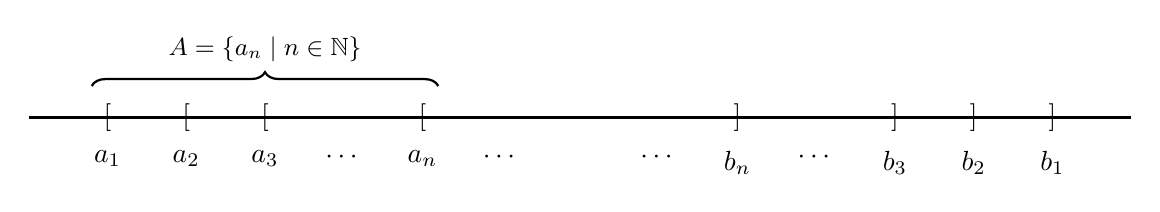
\begin{tikzpicture}
    \draw[thick] (-7, 0) -- (7, 0);

    \foreach \i/\pos in {1/-6, 2/-5, 3/-4, n/-2} {
      \node at (\pos, 0) {$[$};
      \node[below] at (\pos, -0.3) {$a_{\i}$};
    }
    \node[below] at (-3, -0.3) {$\cdots$};

    \foreach \i/\pos in {n/2, 3/4, 2/5, 1/6} {
      \node at (\pos, 0) {$]$};
      \node[below] at (\pos, -0.3) {$b_{\i}$};
    }
    \node[below] at (3, -0.3) {$\cdots$};

    \node[below] at (1, -0.3) {$\cdots$};
    \node[below] at (-1, -0.3) {$\cdots$};

    \draw[decorate,decoration={brace,amplitude=5pt},thick] (-6.2, 0.4) -- (-1.8, 0.4) node[midway, above=5pt] {{\small$A = \{a_n \mid n \in \N\}$}};
  \end{tikzpicture}
\end{figure}

\begin{example}\leavevmode
  \begin{enumerate}
    \item The interval $I_n = \left[0, \frac{1}{n}\right]$, which is clearly $I_n \supset I_{n+1}$, since $\bigcap_{n=1}^\infty = \{0\}$.

    \item The counter example is $I_n = \left(0, \frac{1}{n}\right)$, $\bigcap_{n=0}^\infty I_n = \emptyset$, since $0 \notin I_n$. \qedhere
  \end{enumerate}
\end{example}


\begin{proposition}
  The set $\N$ is unbounded.
\end{proposition}

\begin{proof}
  Assume, for contradiction, that $\N$ is bounded above. Then, it follows that we can set $\alpha = \sup(\N)$. If we consider $\alpha - 1$, then we no longer have an upper bound for $\N$, and therefore, there exists an $n \in \N$ satisfying $\alpha - 1 < n$, which is equivalent to $\alpha < n + 1$. Since we have $n + 1 \in \N$, this contradicts the assumption that $\alpha$ is the least upper bound of $\N$.
\end{proof}

\begin{theorem}[Archimedian Property]\leavevmode
  \begin{enumerate}
    \item $(\forall x \in \R)(\exists n \in \N)[n > x]$.

    \item $(\forall y > 0)(\exists n \in \N)[\sfrac{1}{n} < 1]$.
  \end{enumerate}
\end{theorem}

\begin{proof}\leavevmode
  \begin{enumerate}
    \item Property (i) follows given that $\N$ is unbounded.

    \item Apply property (i) with $x = \sfrac{1}{y} > 0$. \qedhere
  \end{enumerate}
\end{proof}

  \lecture{4}{Oct 7 2024 Mon (13:01:52)}{Consequences of Completeness}

% \subsection{Nested Interval Property}

% \begin{theorem}[Nested Interval Property]
%   For each $n \in \N$, assume we are given a closed interval $I_n = [a_n, b_n] = \left\{x \in \R \mid a_n \le x \le b_n\right\}$. Assume also that each $I_n$ contains the next interval, i.e., $I_n \supseteq I_{n+1}$. Then, the resulting sequence of closed intervals
%   \[%
%     I_1 \supseteq I_2 \supseteq I_3 \supseteq \cdots
%   ,\]%
%   has a nonempty intersection. That is,
%   \[%
%     \bigcap_{n=1}^\infty I_n \neq \emptyset
%   .\]%
% \end{theorem}

% \begin{proof}
%   Let $A = \{a_n : n \in \N\}$. Since $I_n \supseteq I_{n+1}$, we have $a_1 \le a_2 \le a_3 \le \cdots$ (the left endpoints are nondecreasing) and $b_1 \ge b_2 \ge b_3 \ge \cdots$ (the right endpoints are nonincreasing). Moreover, for each $n$ we have $a_n \le b_n \le b_1$, so $A$ is bounded above by $b_1$.

%   By the Axiom of Completeness, $A$ has a least upper bound $s = \sup(A)$. Combining these inequalities, for every $n$ we have
%   \[%
%     a_n \le s \le b_n
%   ,\]%
%   which means $s \in I_n$ for all $n \in \N$. Hence
%   \[%
%     s \in \bigcap_{n=1}^\infty I_n
%   ,\]%
%   proving that the intersection is nonempty.
% \end{proof}

% The Nested Interval Property can be viewed graphically, as shown below.
% \begin{figure}[H]
%   \centering

%   \begin{tikzpicture}
%     \draw[thick] (-7, 0) -- (7, 0);

%     \foreach \i/\pos in {1/-6, 2/-5, 3/-4, n/-2} {
%       \node at (\pos, 0) {$[$};
%       \node[below] at (\pos, -0.3) {$a_{\i}$};
%     }
%     \node[below] at (-3, -0.3) {$\cdots$};

%     \foreach \i/\pos in {n/2, 3/4, 2/5, 1/6} {
%       \node at (\pos, 0) {$]$};
%       \node[below] at (\pos, -0.3) {$b_{\i}$};
%     }
%     \node[below] at (3, -0.3) {$\cdots$};

%     \node[below] at (1, -0.3) {$\cdots$};
%     \node[below] at (-1, -0.3) {$\cdots$};

%     \draw[decorate,decoration={brace,amplitude=5pt},thick] (-6.2, 0.4) -- (-1.8, 0.4) node[midway, above=5pt] {{\small$A = \{a_n \mid n \in \N\}$}};
%   \end{tikzpicture}
% \end{figure}

% \begin{example}\leavevmode
%   \begin{enumerate}
%     \item The interval $I_n = \left[0, \frac{1}{n}\right]$, which is clearly $I_n \supset I_{n+1}$, since $\bigcap_{n=1}^\infty = \{0\}$.

%     \item The counter example is $I_n = \left(0, \frac{1}{n}\right)$, $\bigcap_{n=0}^\infty I_n = \emptyset$, since $0 \notin I_n$. \qedhere
%   \end{enumerate}
% \end{example}


% \begin{proposition}
%   The set $\N$ is unbounded.
% \end{proposition}

% \begin{proof}
%   Assume, for contradiction, that $\N$ is bounded above. Then, it follows that we can set $\alpha = \sup(\N)$. If we consider $\alpha - 1$, then we no longer have an upper bound for $\N$, and therefore, there exists an $n \in \N$ satisfying $\alpha - 1 < n$, which is equivalent to $\alpha < n + 1$. Since we have $n + 1 \in \N$, this contradicts the assumption that $\alpha$ is the least upper bound of $\N$.
% \end{proof}

% \begin{theorem}[Archimedian Property]\leavevmode
%   \begin{enumerate}
%     \item $(\forall x \in \R)(\exists n \in \N)[n > x]$.

%     \item $(\forall y > 0)(\exists n \in \N)[\sfrac{1}{n} < 1]$.
%   \end{enumerate}
% \end{theorem}

% \begin{proof}\leavevmode
%   \begin{enumerate}
%     \item Property (i) follows given that $\N$ is unbounded.

%     \item Apply property (i) with $x = \sfrac{1}{y} > 0$. \qedhere
%   \end{enumerate}
% \end{proof}

% % \section{Density of $\Q$ in $\R$}

% % \begin{theorem}[Density of $\Q$ in $\R$]
% %   Between any two real numbers $a$ and $b$ with $a < b$, there exists a rational number $q$ such that $a < q < b$.
% % \end{theorem}

% % \begin{proof}
% %   Let $a > 0$, giving us $0 < a < b$. Then, $b - a > 0$. By the archimedean property, $(\exists n \in \N)[\sfrac{1}{n} < b - a \iff a < b - \sfrac{1}{n}]$.

% %   There is an $m \in \N$ such that $m - 1 \le na \le m \iff \frac{m - 1}{n} \le a \le \frac{m}{n}$.

% %   On the right hand side, we have $a \le \sfrac{m}{n}$, and on the left hand side, we have
% %   \begin{align*}
% %     \phantom{\implies}\quad&m \le an + 1 \\
% %     \implies\quad&\frac{m}{n} \le b \\
% %     \iff\quad&a \le \frac{m}{n} \le b
% %   .\qedhere\end{align*}
% % \end{proof}

% % Essentially, there are an infinite number of rational numbers between any two real numbers, giving us
% % \[%
% %   a < r_1 < r_2 < r_3 < \dots < b
% % .\]%

% % \begin{corollary}
% %   Between any two real numbers $a < b$, then there are infinitely many irrational numbers.
% % \end{corollary}

% % \begin{proof}
% %   Assume $a > 0$. Given $a < b$, then $a - \sqrt{2} < b - \sqrt{2}$. By the density of $\Q$, then there exists $r \in \Q$ such that $a - \sqrt{2} < r_1 < b - \sqrt{2} \implies a < r + \sqrt{2} < b$. Since $r$ is rational, then $r + \sqrt{2}$ is irrational.
% % \end{proof}

% % \section{Square Roots}

% % \begin{proposition}
% %   There exists a real number $\alpha$ satisfying $\alpha^2 = 2$.
% % \end{proposition}

% % \begin{proof}
% %   Let $S = \left\{x \in \R \mid x^2 < 2\right\}$. Then $S$ is bounded, nonempty, and has a least upper bound. Let $\alpha = \sup(S)$. We want to show $\alpha^2 = 2$ by showing that $\alpha^2 \nless 2$ and $\alpha^2 \ngtr 2$.

% %   \textbf{Case 1} ($\alpha^2 \nless 2$): Suppose $\alpha^2 < 2$. We consider
% %   \begin{align*}
% %     \left(\alpha + \frac{1}{n}\right)^2 &= \alpha^2 + \frac{2\alpha}{n} + \frac{1}{n^2} \\
% %                                         &< \alpha^2 + \frac{2\alpha + 1}{n}
% %   .\end{align*}
% %   Since $\alpha^2 < 2$, we can choose $n$ large enough such that
% %   \[%
% %     \alpha^2 + \frac{2\alpha + 1}{n} < 2 \iff 0 < \frac{2\alpha + 1}{2 - \alpha^2} < n
% %   .\]%
% %   By the archimedian property, there is an $n \in \N$ such that
% %   \[%
% %     \left(\alpha + \frac{1}{n}\right)^2 < 2 \implies \alpha + \frac{1}{n} \in S
% %   ,\]%
% %   but $\alpha$ is the least upper bound, which is a contradiction. Therefore, $\alpha \nless 2$.

% %   \textbf{Case 2} ($\alpha^2 \ngtr 2$): Suppose $\alpha^2 > 2$. We consider
% %   \begin{align*}
% %     \left(\alpha - \frac{1}{n}\right)^2 &= \alpha^2 - \frac{2\alpha}{n} + \frac{1}{n^2} \\
% %                                         &> \alpha^2 - \frac{2\alpha}{n}
% %   .\end{align*}
% %   Since $\alpha^2 > 2$, we can choose $n$ large enough such that
% %   \[%
% %     \alpha^2 - \frac{2\alpha}{n} > 2 \iff 0 < \frac{2\alpha}{\alpha^2 - 2} < n
% %   .\]%
% %   By the archimedian property, there is an $n \in \N$ such that
% %   \[%
% %     \left(\alpha - \frac{1}{n}\right)^2 > 2 \implies \alpha - \frac{1}{n} \notin S
% %   ,\]%
% %   but $\alpha$ is the least upper bound, which is a contradiction. Therefore, $\alpha \ngtr 2$.
% % \end{proof}

  \lecture{5}{Oct 9 2024 Wed (13:02:05)}{}

  % notes end 1-5

  \chapter{Sequences and Series}
  \label{chap:sequences_and_series}

  % notes start 6-13
  \nte[Section 2.2]{Oct 14 2024 Mon (13:00:26)}{Limit of a Sequence}

\section{Required Definitions}
\label{sec:required_definitions}

\begin{definition}
  A \textit{sequence} is a function whose domain is $\N$.
\end{definition}

Given a function $f : \N \to \R$, $f(n)$ is just the $n$th term on the list.

\begin{example}
  Each of the following are common ways to describe sequences.
  \begin{enumerate}
    \item $(1, \frac{1}{2}, \frac{1}{3}, \frac{1}{4}, \dots)$.

    \item $(\frac{1 + n}{n})_{n=1}^{\infty} = (\frac{2}{1}, \frac{3}{2},
      \frac{4}{5}, \dots)$.

    \item $(a_n)$, where $a_n = 2^n$ for each $n \in \N$.

    \item $(x_n)$, where $x_1 = 2$ and $x_{n+1} = \frac{x_n + 1}{2}$.
  \end{enumerate}
\end{example}

\begin{definition}[Convergence of a Sequence]
  A sequence $(a_n)$ \textit{converges} to a real number $\ell$ if,
  \[%
    (\forall \epsilon > 0)(\exists N \in \N)(\forall n \ge N) \lvert a_n - \ell \rvert < \epsilon
  .\]%
  We say that $\ell$ is the limit of $(a_n)$.
\end{definition}

One way to think of $(\exists N \in \N)(\forall n \ge N)$ as saying ``eventually
always'', or as ``from some point on''. So, the definition means, if $a_n \to
\ell$, then given any $\epsilon$, then eventually, everything in the sequence is
within $\epsilon$ of $\ell$. You may know this as $\lim_{n \to \infty} a_n = a$.
This is a more formal definition of the limit of a sequence.

\begin{definition}
  Given a real number $a \in \R$ and an $\epsilon > 0$, the set
  \[%
    V_{\epsilon} (a) = \{x \in \R \mid \lvert x - a \rvert < \epsilon\}
  ,\]%
  is called the \textit{$\epsilon$-neighborhood} of $a$.
\end{definition}

The $V_{\epsilon}(a)$ is just an interval centered at $a$ with radius
$\epsilon$.
\begin{figure}[H]
  \centering

  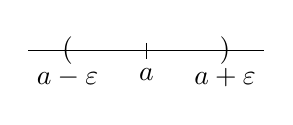
\begin{tikzpicture}
    \draw (-1.5, 0) -- (1.5, 0);

    \node[below=3pt] at (-1, 0) {$a - \epsilon$};
    \node at (-1, 0) {$($};

    \node[midway,below=3pt] at (0, 0) {$a$};
    \draw (0, 0.1) -- (0, -0.1);

    \node[below=3pt] at (1, 0) {$a + \epsilon$};
    \node at (1, 0) {$)$};
  \end{tikzpicture}
\end{figure}

Using the $V_{\epsilon}(a)$ definition, $(a_n)$ converges if, at a certain point
$k$, every term after $k$ is in the $\epsilon$-neighborhood of $a$.

We can re-write the definition of convergence as follows using a topological
version instead of a more numerical analysis way as follows
\begin{definition}[Convergence of a Sequence: Topological Version]
  A sequence $(a_n)$ converges to $a$ if, given any $\epsilon$-neighborhood
  $V_{\epsilon}(a)$ of $a$, there exists a point in the sequence after which all
  of the terms are in $V_{\epsilon}(a)$. In other words, every
  $\epsilon$-neighborhood contains all but a finite number of the terms of
  $(a_n)$.
\end{definition}

\begin{figure}[H]
  \centering

  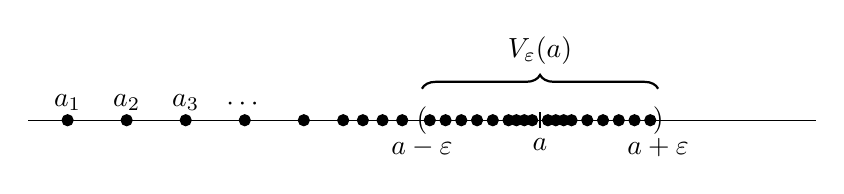
\begin{tikzpicture}
    \draw (-5, 0) -- (5, 0);

    \node[below=3pt] at (0, 0) {$a - \epsilon$};
    \node at (0, 0) {$($};

    \node[below=3pt] at (1.5, 0) {$a$};
    \draw (1.5, 0.1) -- (1.5, -0.1);

    \node[below=3pt] at (3, 0) {$a + \epsilon$};
    \node at (3, 0) {$)$};

    % Outside the interval
    \draw[soldot,above=5pt] (-4.5, 0) circle (2pt) node[above] {$a_1$};
    \draw[soldot,above=5pt] (-3.75, 0) circle (2pt) node[above] {$a_2$};
    \draw[soldot,above=5pt] (-3, 0) circle (2pt) node[above] {$a_3$};
    \draw[soldot,above=5pt] (-2.25, 0) circle (2pt) node[above] {$\cdots$};
    \draw[soldot,above=5pt] (-1.5, 0) circle (2pt);
    \draw[soldot,above=5pt] (-1, 0) circle (2pt);
    \draw[soldot,above=5pt] (-0.75, 0) circle (2pt);
    \draw[soldot,above=5pt] (-0.50, 0) circle (2pt);
    \draw[soldot,above=5pt] (-0.25, 0) circle (2pt);

    % Inside the interval
    \draw[soldot,above=5pt] (0.1, 0) circle (2pt);
    \draw[soldot,above=5pt] (0.3, 0) circle (2pt);
    \draw[soldot,above=5pt] (0.5, 0) circle (2pt);
    \draw[soldot,above=5pt] (0.7, 0) circle (2pt);
    \draw[soldot,above=5pt] (0.9, 0) circle (2pt);
    \draw[soldot,above=5pt] (1.1, 0) circle (2pt);
    \draw[soldot,above=5pt] (1.2, 0) circle (2pt);
    \draw[soldot,above=5pt] (1.3, 0) circle (2pt);
    \draw[soldot,above=5pt] (1.4, 0) circle (2pt);

    \draw[soldot,above=5pt] (1.6, 0) circle (2pt);
    \draw[soldot,above=5pt] (1.7, 0) circle (2pt);
    \draw[soldot,above=5pt] (1.8, 0) circle (2pt);
    \draw[soldot,above=5pt] (1.9, 0) circle (2pt);
    \draw[soldot,above=5pt] (2.1, 0) circle (2pt);
    \draw[soldot,above=5pt] (2.3, 0) circle (2pt);
    \draw[soldot,above=5pt] (2.5, 0) circle (2pt);
    \draw[soldot,above=5pt] (2.7, 0) circle (2pt);
    \draw[soldot,above=5pt] (2.9, 0) circle (2pt);

    \draw[decorate,decoration={brace,amplitude=5pt},thick] (0, 0.4) -- (3, 0.4) node[midway, above=5pt] {$V_{\epsilon}(a)$};
  \end{tikzpicture}
\end{figure}

Both definitions are equivalent. The topological version is more general and
applies to more than just sequences. It should be apparent that the value of $N$
depends on the choice of $\epsilon$. The smaller the $\epsilon$-neighborhood,
the larger $N$ may need to be.

% section required_definitions (end)

\section{Working with Limits}
\label{sec:working_with_limits}

\subsection{Quantifiers}
\label{sub_sec:quantifiers}

The definition begins with $(\forall \epsilon > 0)$. This means that we are
trying to prove that the sequence converges for all $\epsilon > 0$. Say,
$\epsilon = 0.00000001$, or $\epsilon = 100000000$, and so on.

The next quantifier is $(\exists N \in \N)$. This means that we need to find a
natural number $N$ such that the condition holds for all $n \ge N$. This doesn't
have to hold for all $N \in \N$, but just one specific value of $N$ will do,
which is typically the hardest part of the proof.

\begin{note}
  The order of the quantifiers is important. In the definition of convergence,
  we have $(\forall \epsilon > 0)(\exists N \in \N)$. This means that $N$ is
  dependent on $\epsilon$. If we had it the other way around, $(\exists N \in
  \N)(\forall \epsilon > 0)$, then we would have to find a single $N$ that works
  for all $\epsilon$, which is not possible.
\end{note}

Here's a template for a proof of $(x_n) \to x$.

\begin{proof} $ $
  \begin{itemize}
    \item ``Let $\epsilon > 0$ be arbitrarily chosen.''

    \item Demonstrate a choice for $N \in \N$. This is the hardest and most time
      consuming part of the proof.

    \item Now, show that $N$ actually works.

    \item ``Assume $n \ge N$.''

    \item You should be able to derive the inequality $\lvert x_n - x \rvert <
      \epsilon$, if your $N$ is chosen well enough. \qedhere
  \end{itemize}
\end{proof}

% subsection quantifiers (end)

\subsection{Examples}
\label{sub_sec:examples}

\begin{question}
  Prove that $(\frac{1}{\sqrt{n}}) \to 0$.
\end{question}

\begin{worksheet}
  Let's first explore the relationship between $\epsilon$ and $N$. Take
  $\epsilon = \sfrac{1}{10}$. This gives us a target zone for the terms in the
  sequence. By claiming that the limit of $(a_n)$ is $0$, we are saying that the
  terms in the sequence get arbitrarily close to $0$. But how close? This is
  where $\epsilon$ comes into play. We want to show that the terms in the
  sequence are within $\sfrac{1}{10}$ of $0$ after a certain point and they stay
  that way, if not get closer.
  The $100$th term $a_{100} = \sfrac{1}{10}$ puts us right on the boundary,
  giving us
  \[%
    \textrm{if}~n > 100, \qtq{then} a_n \in \left(-\frac{1}{10}, \frac{1}{10}\right)
  .\]%
  As you can see, the smaller we choose $\epsilon$, the larger we'll have to
  make $n$. Now, let's try and find $N$ for all $\epsilon > 0$.
  \begin{note}
    \textit{We aren't using a fixed $\epsilon$, since, say $\epsilon =
    \sfrac{1}{10}$, then $N > 100$, say $N = 101$, and were done, so that's just
    trivial}
  \end{note}
  We have the inequality
  \[%
    \frac{1}{\sqrt{N}} < \epsilon \implies \sqrt{N} > \frac{1}{\epsilon} \implies N > \frac{1}{\epsilon^2}
  .\]%
  Now that' we've chosen our $N$, we can finalize and formalize our proof,
  giving us the following.
\end{worksheet}

\begin{proof}
  Let $\epsilon > 0$ be arbitrarily chosen. Choose a natural number $N$
  satisfying
  \[%
    N > \frac{1}{\epsilon^2}~\left(\textrm{say}~N = \max\left\{\left\lfloor \frac{1}{\epsilon^2} \right\rfloor + 1, 0\right\}~\right)
  .\]%
  We now verify that this choice of $N$ has the desired property. Let $n \ge N$.
  Then,
  \[%
    n > \frac{1}{\epsilon^2} \implies \frac{1}{n} < \epsilon^2 \implies \frac{1}{\sqrt{n}} < \epsilon \qtq{hence} \lvert a_n - 0 \rvert < \epsilon
  .\qedhere\]%
\end{proof}

\begin{question}
  Prove that $\displaystyle\lim_{n \to \infty} \frac{2n + 1}{5n + 4} = \frac{2}{5}$.
\end{question}

\begin{worksheet}
  In order to find an $N \in \N$ that satisfies the definition of convergence,
  we need to find a relationship between $\epsilon$ and $N$. Let's first try
  to solve for $n$ in the inequality $\lvert a_n - a \rvert < \epsilon$.
  \[%
    \left\lvert \frac{2n + 1}{5n + 4} - \frac{2}{5} \right\rvert = \frac{3}{5(5n + 4)}
  .\]%
  Now, we can go ahead and solve for $n$, to get
  \[%
    \frac{3}{5(5n + 4)} < \epsilon \implies \frac{5(5n + 4)}{3} < \frac{1}{\epsilon} \implies n > \frac{3}{25\epsilon} - \frac{4}{5}
  .\]%
  Therefore, we can chose
  \[%
    N > \frac{3}{25\epsilon} - \frac{4}{5}~\left(\textrm{say}~N = \max\left\{\left\lfloor \frac{3}{25\epsilon} - \frac{4}{5} \right\rfloor + 1, 0\right\}~\right)
  .\]%
  Now, all that's left is to show that this $N$ works, and we're done.
\end{worksheet}

\begin{proof}
  Let $\epsilon > 0$ be arbitrarily chosen. Choose a natural number $N$ such
  \[%
    N > \frac{3}{25\epsilon} - \frac{4}{5}
  .\]%
  Assume $n > N > 0$. Then,
  \[%
    \lvert a_n - a \rvert = \left\lvert \frac{2n + 1}{5n + 4} - \frac{2}{5} \right\rvert = \frac{3}{5(5n + 4)} < \frac{3}{5(5N + 4)} = \frac{3}{5\left(5\left(\frac{3}{25\epsilon} - \frac{4}{5}\right) + 4\right)} = \frac{3}{5\left(\frac{3}{5\epsilon}\right)} = \epsilon
  .\qedhere\]%
\end{proof}

\begin{theorem}[Uniqueness of Limits]
  The limit of a sequence, when it exists, must be unique.
\end{theorem}

\begin{worksheet}
  We know that $(a_n) \to a$, meaning that there exists $N_1 \in \N$ such that
  $\lvert a_n - a \rvert < \epsilon$ for all $n \ge N_1$. Same thing for $(b_n)
  \to b$. But how do we show that $a = b$?

  Choose $N > \max(\{N_1, N_2\})$. We just let $N$ be the biggest of the two
  $N$'s from the two sequences. We can assume that $n > N$.

  And then just use the triangle inequality to show that $a = b$.
  \[%
    \lvert a - b \rvert = \lvert a - a_n + a_n - b \rvert \le \lvert a - a_n \rvert + \lvert a_n - b \rvert < \epsilon + \epsilon = 2\epsilon
  .\]%
  Some people don't like the fact that everything is less than $2\epsilon$. To
  show that it's less than $\epsilon$, we can let $\lvert a_n - a \rvert <
  \sfrac{\epsilon}{2}$. Same thing for $(b_n)$. Using that, we get the new
  inequality
  \[%
    \lvert a - b \rvert < \frac{\epsilon}{2} + \frac{\epsilon}{2} = \epsilon
  .\]%
  Formalizing it, we get the following proof.
\end{worksheet}

\begin{proof}
  Let $\epsilon > 0$ be arbitrarily chosen. Since $(a_n) \to a$, there exists
  $N_1 \in \N$ such that $\lvert a_n - a \rvert < \sfrac{\epsilon}{2}$ for all
  $n \ge N_1$. Similarly, since $(a_n) \to b$, there exists $N_2 \in \N$ such
  that $\lvert a_n - b \rvert < \sfrac{\epsilon}{2}$ for all $n \ge N_2$. Let $N
  = \max(\{N_1, N_2\})$. Then, for all $n \ge N$,
  \[%
    \lvert a - b \rvert = \lvert a - a_n + a_n - b \rvert \le \lvert a - a_n \rvert + \lvert a_n - b \rvert < \frac{\epsilon}{2} + \frac{\epsilon}{2} = \epsilon
  .\]%
  Since $\epsilon > 0$ was arbitrary, we have $\lvert a - b \rvert = 0$, which
  implies $a = b$.
\end{proof}

This can be re-written as, if $(a_n) \to a$ and $(a_n) \to b$, then $a = b$.

% subsection examples (end)

% section working_with_limits (end)

\newpage

  \nte[Section 2.3]{Oct 16 2024 Wed (13:01:48)}{Algebraic and Order Limit Theorem}

\begin{definition}[Bounded]
  A sequence $(x_n)$ is \textit{bounded} if there exists a number $M > 0$ such
  that $\lvert x_n \rvert \le M$ for all $n \in \N$.
\end{definition}

Geometrically, this means that we can find an interval $[-M, M]$ that contains
every term in the sequence $(x_n)$.

\begin{theorem}
  Every convergent sequence is bounded.
\end{theorem}

\newpage

  \lecture{8}{Oct 16 2024 Wed (13:02:05)}{Algebraic and Order Limit Theorems}

\subsection{Algebraic Limit Theorem}

\begin{definition}[Bounded]
  A sequence $(x_n)$ is \emph{bounded} if there exists a number $M > 0$ such that $|x_n| \le M$ for all $n \in \N$.
\end{definition}

Geometrically, this means that we can find an interval $[-M, M]$ that contains every term in the sequence $(x_n)$.

\begin{theorem}
  Every convergent sequence is bounded.
\end{theorem}

\begin{worksheet}
  Given $(a_n)$, we need to show that if $\lim_{n \to \infty} a_n = a$, then $(a_n)$ is bounded. Using the definition of a limit, $(\forall \epsilon > 0)(\exists N \in \N)(\forall n > N)[|a_n - a| < \epsilon]$. Expanding the inequality using \ref{eq:triangle_inequality}, we get
  \[%
    |a_n| = |a_n - a + a| \le |a_n + a| - |a| < \epsilon + |a|
  .\]%
  We then can let $M$ be the biggest number in the set $\{|a_1|, |a_2|, \cdots, |a_n|, |a| + \epsilon\}$. Then, that means that every term in the sequence $(a_n)$ is less than or equal to $M$, so $(a_n)$ is bounded.
\end{worksheet}

\begin{proof}
  For $\epsilon > 1$, there exists an $N \in \N$ such that for all $n > N$, $|a_n - a| < \epsilon$. Then, by the triangle inequality, we have
  \[%
    |a_n| = |a_n - a + a| \le |a_n - a| + |a| < \epsilon + |a|
  .\]%
  We let $M = \max(\{|a_1|, |a_2|, \cdots, |a_n|, |a| + \epsilon \})$. Then, $(\forall n \in \N)[|a_n| \le M]$, implying that $(a_n)$ is bounded.
\end{proof}

\begin{theorem}[Algebraic Limit Theorem]
  Let $\lim_{n \to \infty} a_n = a$, and $\lim_{n \to \infty} b_n = b$. Then,
  \begin{enumerate}
    \item $\lim_{n \to \infty} (ca_n) = ca$, for all $c \in \R$.

    \item $\lim_{n \to \infty} (a_n + b_n) = a + b$.

    \item $\lim_{n \to \infty} (a_nb_n) = ab$.

    \item $\lim_{n \to \infty} \frac{a_n}{b_n} = \frac{a}{b}$, provided that $b
      \ne 0$.
  \end{enumerate}
\end{theorem}

\begin{proof}\leavevmode
  \begin{enumerate}
    \item Let $\epsilon > 0$. Then, there exists an $N \in \N$ such that for all $n > N$, $|a_n - a| < \frac{\epsilon}{|c|}$. Then, we have
      \[%
        |ca_n - ca| = |c| \cdot |a_n - a| < |c| \cdot \frac{\epsilon}{|c|} = \epsilon
      .\]%

    \item Let $\epsilon > 0$. Then, there exists an $N \in \N$ such that for all $n > N$, $|a_n - a| < \frac{\epsilon}{2}$ and $|b_n - b| < \frac{\epsilon}{2}$. Then, we have
      \[%
        |(a_n + b_n) - (a + b)| = |(a_n - a) + (b_n - b)| \le |a_n - a| + |b_n - b| < \frac{\epsilon}{2} + \frac{\epsilon}{2} = \epsilon
      .\]%

    \item Let $\epsilon > 0$. Observe the fact that
      \begin{align*}
        |a_nb_n - ab| &= |a_nb_n - ab_n + ab_n - ab| \\
                                  &\le |a_nb_n - ab_n| + |ab_n - ab| \\
                                  &= |b_n| \cdot |a_n - a| + |a| \cdot |b_n - b|
      .\end{align*}
      Since $(b_n)$ converges, that means it's bounded by some $M > 0$. Then, we have
      \[%
        |b_n| \cdot |a_n - a| + |a| \cdot |b_n - b| \le M \cdot |a_n - a| + |a| \cdot |b_n - b|
      .\]%
      Choose an $N_1$ and $N_2$ such that
      \[%
        (\forall n \ge N_1)\left[|b_n - b| < \frac{1}{|a|} \cdot \frac{\epsilon}{2}\right] \aand (\forall n \ge N_2)\left[|a_n - a| < \frac{1}{M} \cdot \frac{\epsilon}{2}\right]
      .\]%
      Pick $N = \max(\{N_1, N_2\})$. If $n \ge N$, then we get
      \begin{align*}
        |a_nb_n - ab| &< M \cdot |a_n - a| + |a| \cdot |b_n - b| \\
                                  &< M \left(\frac{\epsilon}{2M}\right) + |a| \cdot \left(\frac{\epsilon}{2 |a|}\right) = \epsilon
      .\end{align*}

    \item Using part (iii), we only need to show that $\lim_{n \to \infty} \frac{1}{b_n} = \frac{1}{b}$. Let $\epsilon > 0$. Observe the fact that
      \[%
        \left|\frac{1}{b_n} - \frac{1}{b} \right\rvert = \frac{|b - b_n|}{|b| \cdot |b_n|}
      .\]%
      Choose $N_1$ and $N_2$ such that
      \[%
        (\forall n \ge N_1)\left[|a_n - b| < \frac{|b|}{2}\right] \aand (\forall n \ge N_2)\left[|b_n - b| < \frac{\epsilon |b|^2}{2}\right]
      .\]%
      Pick $N = \max(\{N_1, N_2\})$, then we get
      \[%
        \left|\frac{1}{b_n} - \frac{1}{b} \right\rvert = |b - b_n| < \frac{\epsilon |b|^2}{2} \cdot \frac{1}{|b| \cdot \frac{|b|}{2}} = \epsilon
      .\qedhere\]%
  \end{enumerate}
\end{proof}

\subsection{Order Limit Theorem}

\begin{theorem}[Order Limit Theorem]
  Assume $\lim_{n \to \infty} a_n = a$ and $\lim_{n \to \infty} b_n = b$.
  \begin{enumerate}
    \item If $a_n \ge 0$ for all $n \in \N$, then $a \ge 0$.

    \item If $a_n \le b_n$ for all $n \in \N$, then $a \le b$.

    \item If there exists $c \in \R$ for which $c \le b_n$ for all $n \in \N$, then $c \le b$. Similarly, if $a_n \le c$ for all $n \in \N$, then $a \le c$.
  \end{enumerate}
\end{theorem}

\begin{proof}\leavevmode
  \begin{enumerate}
    \item Assume $a < 0$. Consider the particular value $\epsilon = |a|$. Then, we can find an $N$ such that $|a_n - a| < |a|$, for all $n \ge N$. This would mean that $|a_N - a| < |a|$, which implies that $a_N < 0$, which contradicts our hypothesis. Therefore, $a \ge 0$

    \item By the Algebraic Limit Theorem, the sequence $(b_n - a_n)$ converges to $b - a$. Because $b_n - a_n > 0$, we can apply part (i) to get $b - a \ge 0$, which implies that $a \le b$.

    \item Take $a_n = c$ or $b_n = c$ in part (ii) to get the desired result. \qedhere
  \end{enumerate}
\end{proof}

Limits and their properties don't depend on the first few terms of the sequence. Changing the value of the first ten or even ten thousand terms doesn't change the limit of the sequence.

  \lecture{9}{Oct 18 2024 Fri (13:02:06)}{Monotone Convergence Theorem}

\begin{definition}[Monotone]
  A sequence $(a_n)$ is \emph{increasing} if $(\forall n \in \N)[a_n \le a_{n+1}]$ and \emph{decreasing} if $(\forall n \in \N)[a_n \ge a_{n+1}]$. A sequence is \emph{monotone} if it is either increasing or decreasing.
\end{definition}

\begin{theorem}[Monotone Convergence Theorem]
  Every bounded monotone sequence converges.
\end{theorem}

\begin{proof}
  Let $\left(a_n\right)$ be monotone and bounded. To prove $\left(a_n\right)$ converges using the definition of convergence, we are going to need a candidate for the limit. Let's assume the sequence is increasing (the decreasing case is handled similarly), and consider the set of points $\{a_n \mid n \in \N\}$. By assumption, this set is bounded, so we can let
  \[%
    s = \sup(\{a_n \mid n \in \N\})
  .\]%
  It seems reasonable to claim that $\lim a_n = s$.

  To prove this, let $\epsilon > 0$. Because $s$ is the least upper bound for $\{a_n \mid n \in \N\}$, $s - \epsilon$ is not an upper bound, so there exists a point in the sequence $a_N$ such that $s - \epsilon < a_N$. Now, the fact that $(a_n)$ is increasing implies that if $n \geq N$, then $a_N \leq a_n$. Hence,
  \[%
    s - \epsilon < a_N \leq a_n \leq s < s + \epsilon
  ,\]%
  which implies $\abs{a_n - s} <\epsilon$, as desired.
\end{proof}

We now have another tool to prove the Nested Interval Property.
\begin{theorem}[Nested Interval Property]
  For each $n \in \N$, assume we are given a closed interval $I_n = [a_n, b_n] = \left\{x \in \R \mid a_n \le x \le b_n\right\}$. Assume also that each $I_n$ contains the next interval, i.e., $I_n \supseteq I_{n+1}$. Then, the resulting sequence of closed intervals
  \[%
    I_1 \supseteq I_2 \supseteq I_3 \supseteq \cdots
  ,\]%
  has a nonempty intersection. That is,
  \[%
    \bigcap_{n=1}^\infty I_n \neq \emptyset
  .\]%
\end{theorem}

\begin{proof}
  Assume we have the following interval $I_n = [a_n, b_n]$ for each $n \in \N$. Since all $I_n \supseteq I_{n+1}$, then we have the following inequality
  \[%
    I_n = [a_n, b_n] \supseteq I_{n+1} = [a_{n+1}, b_{n+1}] \implies \begin{cases*}
      a_n \le a_{n+1} \\
      b_n \ge b_{n+1}
    \end{cases*}
  .\]%
  This means that $(a_n)$ is bounded by $b_1$ from above and $(b_n)$ is bounded by $a_1$ from below. Then, by the MCT, $(a_n)$ converges to $a$ and $(b_n)$ converges to $b$. Hence,
  \[%
    [a, b] \in \bigcap_{n=1}^\infty I_n
  .\qedhere\]%
\end{proof}

\begin{question}
  Let $S_1 = 1$ and $S_{n+1} = \sqrt{S_n + 1}$, for $n \ge 1$. Show $S_n$ converges and find the limit.
\end{question}

\begin{proof}[Solution]
  Let's find the first few terms of the sequence
  \[%
    S_1 = 1, \quad S_2 = \sqrt{2}, \quad S_3 = \sqrt{\sqrt{2} + 1}, \quad S_4 = \sqrt{\sqrt{\sqrt{2} + 1} + 1}
  .\]%
  Then, we get the following inequality
  \[%
    S_1 < S_2 < S_3 < S_4 < \cdots
  .\]%

  We can then use induction to show that $S_n < S_{n+1}$ for all $n \in \N$ and then show that the sequence is bounded. Then, we can conclude by the MTC that the sequence must converge.

  Using induction, assume $S_{n-1} \le S_n$. Now, we show that $S_n \le S_{n+1}$. We have
  \begin{align*}
    S_{n+1} - S_n &= \sqrt{S_n + 1} - \sqrt{S_{n-1} + 1} \\
                  &= \frac{(S_n + 1) - (S_{n-1} + 1)}{\sqrt{S_n + 1} + \sqrt{S_{n-1} + 1}} \\
                  &= \frac{S_n - S_{n-1}}{\sqrt{S_n + 1} + \sqrt{S_{n-1} + 1}} \ge 0
  .\end{align*}
  Therefore, $S_n \le S_{n+1}$ for all $n \in \N$, meaning that $S_n$ is increasing.

  We now show that $S_n$ is bounded. Assume $S_n \le 2$. Then $S_{n+1} = \sqrt{S_n + 1} \le \sqrt{2 + 1} = \sqrt{3} \le \sqrt{2}$.

  Hence, by induction, $S_n \le 2$ for all $n$. So, $(S_n)$ is an increasing bounded sequence. By MCT, $(S_n)$ converges to $L$.

  Now, all that's left is to find the limit of the sequence.
  \[%
    \lim_{n \to \infty} S_n = \lim_{n \to \infty} S_{n+1} = S \implies S = \sqrt{S + 1} \implies S^2 = S + 1
  .\]%
  Solving the equation using the quadratic equation, we get
  \[%
    S = \frac{1 \pm \sqrt{5}}{2}
  .\]%
  But, as we've seen before, the limit value of a sequence is always unique. So, how do we choose which one the limit is? We'll, it must be the positive term, since $S_n \ge 1$ for all $n \in \N$. Therefore, the limit of the sequence is
  \[%
    \lim_{n \to \infty} S_n = \frac{1 + \sqrt{5}}{2}
  .\qedhere\]%
\end{proof}

  \lecture{10}{Oct 23 2024 Wed (13:00:51)}{Intro to Infinite Series}

\section{Infinite Series}
\label{sec:infinite_series}

\begin{definition}[Infinite Series and Partial Sums]
  Let $b_n$ be a sequence. An \textit{infinite series} is a formal expression of
  the form
  \[%
    \sum_{n=1}^{\infty} b_n = b_1 + b_2 + b_3 + \cdots
  .\]%
  The $n$-th \textit{partial sum} of the series s
  \[%
    s_m = \sum_{n=1}^{m} b_n = b_1 + b_2 + \cdots + b_m
  .\]%
\end{definition}

If $(b_n)$ converges to $L$, then we say $\sum_{n=1}^{\infty} b_n$ converges.
The following are equivalent
\[%
  \lim_{n \to \infty} s_n = L = \lim_{n \to \infty} \sum_{k=1}^n b_k
.\]%

\begin{theorem}
  If $(\forall n \in \N)[a_n \ge 0]$, then $\sum_{n=1}^{\infty} a_n$ converges
  if and only if the sequence of partial sums $(s_n)$ is bounded.
\end{theorem}

\begin{proof}
  If $a_n \ge 0$, then $s_{n+1} = s_n + a_n \ge s_n$. By the Monotone
  Convergence Theorem, $(s_n)$ converges if and only if it is bounded.
\end{proof}

\begin{example}
  Given the sequence $a_n = \frac{1}{n^2}$. We can re-write this as
  \[%
    \sum_{n=1}^N \frac{1}{n^2} = 1 + \sum_{n=2}^N \frac{1}{n^2}
  .\]%
  This gives us
  \begin{align*}
    n^2 &\ge n(n - 1) \\
        &< 1 + \sum_{n=2}^N \frac{1}{n(n - 1)} = 1 + \sum_{n=2}^N \left(\frac{1}{n - 1} - \frac{1}{n}\right) \\
        &= 1 + \left(1 - \frac{1}{N}\right) = 2 - \frac{1}{N} < 2
  .\end{align*}
  So, $n^2 \ge 2$ for all $n \in \N$. Thus, $a_n = \frac{1}{n^2}$ is bounded
  below by $0$ and above by $2$. Therefore, $\sum_{n=1}^{\infty} \frac{1}{n^2}$
  converges.
\end{example}

% section infinite_series (end)

  \lecture{11}{Oct 28 2024 Mon (13:03:26)}{More Advanced Infinite Series}

  \lecture{12}{Oct 28 2024 Mon (13:00:12)}{Subsequences}

\begin{definition}[Subsequence]
  Let $(a_n)$ be a sequence and $(n_k)$ be a strictly increasing sequence of natural numbers. Then, the sequence $(a_{n_k}) = (a_{n_1}, a_{n_2}, \dots)$ is called a \emph{subsequence of $(a_n)$}.
\end{definition}

\begin{example}
  The sequence $(n)$ contains the subsequences $(2^n)$, $(2n)$, and $(n^2)$.
\end{example}

Now, a bunch of questions arise. If $(a_n)$ is a bounded sequence, can it have a convergent subsequence? If $(a_n)$ is an unbounded sequence, can it have a bounded sequence? For now, I'll answer the question if all subsequences of a convergent sequence converge to the same limit.

\begin{theorem}
  If $(a_n)$ is a convergent sequence, then all its subsequences converge to the same limit.
\end{theorem}

\begin{proof}
  Let $\epsilon > 0$. There is an $N \in \N$ such that for all $n > N$, $\lvert a_n - a \rvert < \epsilon$.

  Let $(a_{n_k})$ be a subsequence. Then, $n_k \ge k$. Hence, $n_N \ge N$. Hence, for all $n_k > n_N$, $\lvert a_{n_k} - a \rvert < \epsilon$.
\end{proof}

\begin{example}
  Let $0 < b < 1$. Since $b > b^2 > b^3 > \cdots > 0$, the sequence $(b^n)$ is decreasing and bounded below by $0$. Hence, by the Monotone Convergence Theorem, $b^n \to l$. Notice that $\left(b^{2n}\right)$ is a subsequence of $\left(b^n\right)$, so $b^{2n} \to l \cdot l = l^2$. Since limits are unique, it follows that $l = 0$. We can then generalize this example to conclude that $b^n \to 0 \iff -1 < b < 1$.
\end{example}

We can use this theorem to prove that a sequence doesn't converge by finding two subsequences that converge to different limits.

\begin{example}[Divergence Criterion]
  Let $(a_n)$ be the sequence defined by
  \[%
    (a_n) = \left(0, \frac{1}{2}, -\frac{1}{2}, \frac{1}{3}, \frac{2}{3}, -\frac{2}{3}, \dots\right)
  .\]%
  Notice that we get three different subsequences
  \[%
    \left(a_{n_1}\right) = \left(0, \frac{1}{2}, \frac{1}{3}, \cdots\right), \quad
    \left(a_{n_2}\right) = \left(0, \frac{1}{2}, \frac{2}{3}, \cdots\right), \aand
    \left(a_{n_3}\right) = \left(0, -\frac{1}{2}, -\frac{2}{3}, \cdots\right)
  .\]%
  The first subsequence converges to $0$, the second subsequence converges to $1$, and the third subsequence converges to $-1$. Hence, the sequence $(a_n)$ doesn't converge.
\end{example}

  \lecture{13}{Oct 30 2024 Wed (13:02:06)}{Rearrangements of Infinite Series}

% \begin{definition}[Rearrangement of a Series]
%   Let $\sum_{n=1}^\infty a_n$ be an infinite series. A \emph{rearrangement} of this series is a series obtained by permuting its terms, that is
%   \[%
%     \sum_{n=1}^\infty a_{\sigma(n)}
%   ,\]%
%   where $\sigma : \N \to \N$ is a bijection (a one-to-one and onto mapping).
% \end{definition}

% \begin{theorem}[Riemann's Rearrangement Theorem]
%   If $\sum_{n=1}^\infty a_n$ is a conditionally convergent series, then for any real number $L \in \R$ (or even $\pm\infty$), there exists a rearrangement $\sigma$ such that,
%   \[%
%     \sum_{n=1}^\infty a_{\sigma(n)} = L
%   .\]%
% \end{theorem}

% \begin{proof}
%   Since $\sum_{n=1}^\infty a_n$ is conditionally convergent, the positive terms $\{a_n^+\}$ and negative terms $\{a_n^-\}$ both diverge to $+\infty$ in absolute value. To construct a rearrangement summing to $L$, proceed as follows.
%   \begin{itemize}
%     \item Select positive terms $\{a_n^+\}$ to sum until the partial sum exceeds $L$.

%     \item Then add negative terms $\{a_n^-\}$ to decrease the partial sum until it falls below $L$.

%     \item Alternate between adding positive and negative terms in this manner, ensuring the partial sums oscillate closer and closer to $L$.
%   \end{itemize}
%   This process guarantees convergence to $L$, as the series' terms tend to zero and the oscillations diminish.
% \end{proof}

% \begin{corollary}
%   If $\sum_{n=1}^\infty a_n$ converges absolutely, then any rearrangement $\sum_{n=1}^\infty a_{\sigma(n)}$ also converges to the same sum,
%   \[%
%     \sum_{n=1}^\infty a_{\sigma(n)} = \sum_{n=1}^\infty a_n
%   .\]%
% \end{corollary}

% \begin{proof}
%   Absolute convergence implies that $\sum_{n=1}^\infty a_n \le \sum_{n=1}^\infty \lvert a_n \rvert \in \R$. Rearranging the terms does not affect the total sum since the series converges uniformly regardless of order.
% \end{proof}

% \begin{example}[Harmonic Series Rearrangements]
%   The harmonic series $\sum_{n=1}^\infty \frac{(-1)^{n+1}}{n}$ converges conditionally to $\ln(2)$. By Riemann’s Rearrangement Theorem, this series can be rearranged to sum to any real number $L$ or diverge to $\pm\infty$.
% \end{example}

% \begin{lemma}[Group Rearrangements]
%   Grouping terms of an absolutely convergent series into blocks does not change its sum. For example, if $a_n = \frac{1}{n^2}$, grouping the terms as $(a_1)$, $(a_2 + a_3)$, $(a_4 + a_5 + a_6)$, etc., preserves the sum,
%   \[%
%     \sum_{n=1}^\infty a_n = \sum_{k=1}^\infty \left( \sum_{j=1}^k a_j \right)
%   .\]%
% \end{lemma}

% \begin{proof}
%   Let $S_n$ denote the partial sums of $\sum_{n=1}^\infty a_n$. Grouping terms corresponds to defining a new sequence of partial sums $T_m$, where $T_m$ involves summing blocks of $S_n$. Since $\sum_{n=1}^\infty a_n$ converges absolutely, $T_m$ converges to the same limit as $S_n$.
% \end{proof}

% \begin{example}[Rearrangement and Divergence]
%   Consider the series $\sum_{n=1}^\infty \frac{1}{n}$, which diverges. Any rearrangement of this series also diverges, as the partial sums tend to infinity regardless of the order of terms.
% \end{example}

% \begin{theorem}[Unordered Series Convergence]
%   If $\sum_{n=1}^\infty a_n$ converges conditionally, the set of all sums obtained by rearranging the series is unbounded. That is, the sums can fill the entire real number line $\R$.
% \end{theorem}

% \begin{proof}
%   By Riemann’s Rearrangement Theorem, for any $L \in \R$, there exists a rearrangement $\sigma$ such that $\sum_{n=1}^\infty a_{\sigma(n)} = L$. This implies that the set of rearranged sums is dense in $\R$ and unbounded.
% \end{proof}

  % notes end 6-13

  \chapter{Basic Topology of $\R$}
  \label{chap:basic_topology_of_r}

  % notes start 14-17
  \lecture{14}{Nov 4 2024 Mon (13:02:06)}{Properties of Infinite Series}

  \lecture{15}{Nov 4 2024 Mon (13:02:06)}{Properties of Series, Rearrangements}

Just as we had an algebraic limit theorem for sequences, we have a similar theorem for series.
\begin{theorem}[Algebraic Limit Theorem for Series]
  If $\sum_{k=1}^\infty a_k = A$ and $\sum_{k=1}^\infty b_k = B$, then
  \begin{enumerate}
    \item $\sum_{k=1}^\infty ca_k = cA$ for all $c \in \R$.

    \item $\sum_{k=1}^\infty (a_k + b_k) = A + B$.
  \end{enumerate}
\end{theorem}

\begin{proof}\leavevmode
  \begin{enumerate}
    \item Let $S_n = \sum_{k=1}^n a_k$. Then, $\lim_{m \to \infty} S_m = A$. Thus, by the Algebraic Limit Theorem for Sequences, $c\lim_{m \to \infty} S_m = \lim_{m \to \infty} (cS_m) = cA$. Thus, $\sum_{k=1}^\infty ca_k = cA$.

    \item Let $S_n = \sum_{k=1}^n a_k$ and $T_n = \sum_{k=1}^n b_k$. Then, $\lim_{m \to \infty} S_m = A$ and $\lim_{m \to \infty} T_m = B$. Thus, by the Algebraic Limit Theorem for Sequences, $\lim_{m \to \infty} (S_m + T_m) = A + B$. Thus, $\sum_{k=1}^\infty (a_k + b_k) = A + B$. \qedhere
  \end{enumerate}
\end{proof}

Just as we had the Cauchy criterion for sequences, we have a similar criterion for series.
\begin{theorem}[Cauchy Criterion for Series]
  The series $\sum_{k=1}^\infty a_k$ converges if and only if, given $\epsilon > 0$, there exists an $N \in \N$ such that whenever $n > m > N$, it follows that
  \[%
    \lvert a_{m+1} + a_{m+2} + \cdots + a_n \rvert < \epsilon
  .\]%
\end{theorem}

\begin{proof}
  Notice that
  \[%
    \left\lvert \sum_{k=1}^n a_k - \sum_{k=1}^m a_k \right\rvert = \lvert S_n - S_m \rvert = \lvert a_{m+1} + a_{m+2} + \cdots + a_n \rvert
  .\]%
  Thus, the series converges if and only if the sequence of partial sums is a Cauchy sequence.
\end{proof}

This is a very powerful criterion. We use this theorem to prove all of the basic tests in the future.

\begin{definition}[Absolute Convergence]
  A series $\sum_{k=1}^\infty a_k$ is said to \emph{converge absolutely} if the series $\sum_{k=1}^\infty \lvert a_k \rvert$ converges.
\end{definition}

\begin{definition}[Conditional Convergence]
  A series $\sum_{k=1}^\infty a_k$ is said to \emph{converge conditionally} if the series $\sum_{k=1}^\infty a_k$ converges, but the series $\sum_{k=1}^\infty \lvert a_k \rvert$ diverges.
\end{definition}

\subsection{Rearrangements of Infinite Series}

\begin{definition}[Rearrangement of a Series]
  Let $\sum_{n=1}^\infty a_n$ be an infinite series. A \emph{rearrangement} of this series is a series obtained by permuting its terms, that is
  \[%
    \sum_{n=1}^\infty a_{\sigma(n)}
  ,\]%
  where $\sigma : \N \to \N$ is a bijection (a one-to-one and onto mapping).
\end{definition}

\begin{theorem}[Riemann's Rearrangement Theorem]
  If $\sum_{n=1}^\infty a_n$ is a conditionally convergent series, then for any real number $L \in \R$ (or even $\pm\infty$), there exists a rearrangement $\sigma$ such that,
  \[%
    \sum_{n=1}^\infty a_{\sigma(n)} = L
  .\]%
\end{theorem}

\begin{proof}
  Since $\sum_{n=1}^\infty a_n$ is conditionally convergent, the positive terms $\{a_n^+\}$ and negative terms $\{a_n^-\}$ both diverge to $+\infty$ in absolute value. To construct a rearrangement summing to $L$, proceed as follows.
  \begin{itemize}
    \item Select positive terms $\{a_n^+\}$ to sum until the partial sum exceeds $L$.

    \item Then add negative terms $\{a_n^-\}$ to decrease the partial sum until it falls below $L$.

    \item Alternate between adding positive and negative terms in this manner, ensuring the partial sums oscillate closer and closer to $L$.
  \end{itemize}
  This process guarantees convergence to $L$, as the series' terms tend to zero and the oscillations diminish.
\end{proof}

\begin{corollary}
  If $\sum_{n=1}^\infty a_n$ converges absolutely, then any rearrangement $\sum_{n=1}^\infty a_{\sigma(n)}$ also converges to the same sum,
  \[%
    \sum_{n=1}^\infty a_{\sigma(n)} = \sum_{n=1}^\infty a_n
  .\]%
\end{corollary}

\begin{proof}
  Absolute convergence implies that $\sum_{n=1}^\infty a_n \le \sum_{n=1}^\infty \lvert a_n \rvert \in \R$. Rearranging the terms does not affect the total sum since the series converges uniformly regardless of order.
\end{proof}

\begin{example}[Harmonic Series Rearrangements]
  The harmonic series $\sum_{n=1}^\infty \frac{(-1)^{n+1}}{n}$ converges conditionally to $\ln(2)$. By Riemann’s Rearrangement Theorem, this series can be rearranged to sum to any real number $L$ or diverge to $\pm\infty$.
\end{example}

\begin{lemma}[Group Rearrangements]
  Grouping terms of an absolutely convergent series into blocks does not change its sum. For example, if $a_n = \frac{1}{n^2}$, grouping the terms as $(a_1)$, $(a_2 + a_3)$, $(a_4 + a_5 + a_6)$, etc., preserves the sum,
  \[%
    \sum_{n=1}^\infty a_n = \sum_{k=1}^\infty \left( \sum_{j=1}^k a_j \right)
  .\]%
\end{lemma}

\begin{proof}
  Let $S_n$ denote the partial sums of $\sum_{n=1}^\infty a_n$. Grouping terms corresponds to defining a new sequence of partial sums $T_m$, where $T_m$ involves summing blocks of $S_n$. Since $\sum_{n=1}^\infty a_n$ converges absolutely, $T_m$ converges to the same limit as $S_n$.
\end{proof}

\begin{example}[Rearrangement and Divergence]
  Consider the series $\sum_{n=1}^\infty \frac{1}{n}$, which diverges. Any rearrangement of this series also diverges, as the partial sums tend to infinity regardless of the order of terms.
\end{example}

\begin{theorem}[Unordered Series Convergence]
  If $\sum_{n=1}^\infty a_n$ converges conditionally, the set of all sums obtained by rearranging the series is unbounded. That is, the sums can fill the entire real number line $\R$.
\end{theorem}

\begin{proof}
  By Riemann’s Rearrangement Theorem, for any $L \in \R$, there exists a rearrangement $\sigma$ such that $\sum_{n=1}^\infty a_{\sigma(n)} = L$. This implies that the set of rearranged sums is dense in $\R$ and unbounded.
\end{proof}

  \lecture{16}{Nov 8 2024 Fri (13:02:06)}{Closure}

  % notes end 14-17

  \chapter{Functional Limits and Continuity}

  % notes start 17-20
  \lecture{17}{Nov 15 2024 Fri (13:03:05)}{Perfect and Connected Sets}

  \lecture{18}{Nov 13 2024 Wed (13:02:06)}{Definition of Functional Limits}

  \lecture{19}{Nov 15 2024 Fri (13:02:06)}{Perfect and Connected Sets}

\subsection{Perfect Sets}

We recall that a \emph{limit point} of a set $E \subseteq \R^n$ is a point $p$ such that every $\epsilon$-neighborhood of $p$ contains a point of $E$ different from $p$ itself (Lecture~14).

\begin{definition}[Perfect Set]
  A set $P \subseteq \R^n$ is \emph{perfect} if it is closed and every point of $P$ is a limit point of $P$.
\end{definition}

Equivalently, $P$ is perfect if $P = P'$, where $P'$ denotes the set of all limit points of $P$.

\begin{remark}
  A few basic observations, we notice that every perfect set is closed, by definition, perfect sets have no isolated points, and the closure of a perfect set is the set itself.
\end{remark}

\begin{examples}\leavevmode
  \begin{enumerate}
    \item $[0,1]$ is perfect. It is closed, and every point is a limit point: interior points because of nearby points on both sides, and endpoints because of points approaching from within the interval.

    \item The standard middle-third Cantor set $C$ is closed, totally disconnected, and has no isolated points -- hence perfect.

    \item $\Q \cap [0,1]$ is not perfect because it is not closed; its closure is $[0,1]$, which \emph{is} perfect.

    \item $[0,1] \cup \{2\}$ is not perfect because $2$ is isolated.

    \item The set
      \[%
        E = \{x \in [0,1] \mid x!\text{is irrational}\}
      ,\]%
      is perfect. It is closed (complement is $\Q \cap [0,1]$, which is open in the subspace topology) and every irrational in $[0,1]$ is a limit point because rationals and irrationals are both dense in $\R$.

    \item The set of all real numbers whose decimal expansions contain only the digits 4 and 7 is perfect. It is closed, and every point can be approached by other such numbers differing only far out in the decimal expansion. \qedhere
  \end{enumerate}
\end{examples}

\begin{theorem}
  A nonempty perfect set is uncountable.
\end{theorem}

\begin{proof}
  If $P$ is perfect and nonempty, then it must be infinite because otherwise it would consist only of isolated points. Let's assume, for contradiction, that $P$ is countable. Thus, we can write
  \[%
    P=\left\{x_1, x_2, x_3, \cdots\right\}
  ,\]%
  where every element of $P$ appears on this list. The idea is to construct a sequence of nested compact sets $K_n$, all contained in $P$, with the property that
  $x_1 \notin K_2, x_2 \notin K_3, x_3 \notin K_4, \cdots$. We can use the Nested
  Compact Set Property to produce an
  \[%
    x \in \bigcap_{n=1}^{\infty} K_n \subseteq P
  ,\]%
  that cannot be on the list $\left\{x_1, x_2, x_3, \cdots\right\}$.

  Let $I_1$ be a closed interval that contains $x_1$ in its interior (i.e., $x_1$ is not an endpoint of $I_1$ ). Now, $x_1$ is not isolated, so there exists some other point $y_2 \in P$ that is also in the interior of $I_1$. Construct a closed interval $I_2$, centered on $y_2$, so that $I_2 \subseteq I_1$ but $x_1 \notin I_2$. More explicitly, if $I_1=[a, b]$, let
  \[%
    \epsilon = \min(\{y_2 - a, b - y_2, |x_1 - y_2|\})
  .\]%

  Then, the interval $I_2 = [y_2 - \epsilon/2, y_2 + \epsilon/2]$ has the desired properties.

  This process can be continued. Because $y_2 \in P$ is not isolated, there must exist another point $y_3 \in P$ in the interior of $I_2$, and we may insist that $y_3 \neq x_2$. Now, construct $I_3$ centered on $y_3$ and small enough so that $x_2 \notin I_3$ and $I_3 \subseteq I_2$. Observe that $I_3 \cap P \neq \emptyset$ because this intersection contains at least $y_3$.

  If we carry out this construction inductively, the result is a sequence of closed intervals $I_n$ satisfying
  \begin{enumerate}
    \item $I_{n+1} \subseteq I_n$,
    \item $x_n \notin I_{n+1}$, and
    \item $I_n \cap P \neq \emptyset$.
  \end{enumerate}

  To finish the proof, we let $K_n = I_n \cap P$. For each $n \in \N$, we have that $K_n$ is closed because it is the intersection of closed sets, and bounded because it is contained in the bounded set $I_n$. Hence, $K_n$ is compact. By construction, $K_n$ is not empty and $K_{n+1} \subseteq K_n$. Thus, we can employ the Nested Compact Set Property to conclude that the intersection
  \[%
    \bigcap_{n=1}^{\infty} K_n \neq \emptyset
  .\]%

  But each $K_n$ is a subset of $P$, and the fact that $x_n \notin I_{n+1}$ leads to the conclusion that $\bigcap_{n=1}^{\infty} K_n = \emptyset$, which is the sought-after contradiction.
\end{proof}

\subsection{Connected Sets}

Intuitively, a set is connected if it is ``all in one piece'' and cannot be split into two nonempty parts that are apart from each other.

\begin{definition}[Connected Set]
  A set $E \subseteq \R^n$ is \emph{connected} if it cannot be expressed as the union $E = U \cup V$ of two disjoint nonempty sets $U$ and $V$ that are open in the relative topology on $E$.
\end{definition}

Equivalently: the only subsets of $E$ that are both open and closed (in the relative topology) are $\emptyset$ and $E$ itself.

\begin{examples}\leavevmode
  \begin{enumerate}
    \item If we let $A=(1,2)$ and $B=(2,5)$, then it is not difficult to verify that $E=(1,2) \cup(2,5)$ is disconnected. Notice that the sets $C=(1,2]$ and $D=(2,5)$ are not separated because $C \cap \bar{D}=\{2\}$ is not empty. This should be comforting. The union $C \cup D$ is equal to the interval $(1,5)$, which better not qualify as a disconnected set. We will prove in a moment that every interval is a connected subset of $\R$ and vice versa.

    \item Let's show that the set of rational numbers is disconnected. If we let
      \[%
        A = \Q \cap(-\infty, \sqrt{2}) \aand B = \Q \cap(\sqrt{2}, \infty)
      ,\]%
      then we certainly have $\Q = A \cup B$. The fact that $A \subseteq(-\infty, \sqrt{2})$ implies (by the Order Limit Theorem) that any limit point of $A$ will necessarily fall in $(-\infty, \sqrt{2}]$. Because this is disjoint from $B$, we get $\bar{A} \cap B = \emptyset$. We can similarly show that $A \cap \bar{B} = \emptyset$, which implies that $A$ and $B$ are separated.
  \end{enumerate}
\end{examples}

\begin{theorem}
  A set $E \subseteq \R$ is connected if and only if, for all nonempty disjoint sets $A$ and $B$ satisfying $E = A \cup B$, there always exists a convergent sequence $(x_n) \to x$ with $(x_n)$ contained in one of $A$ or $B$, and $x$ an element of the other.
\end{theorem}

\begin{proof}
  We use the usual topological definition: $E$ is \emph{connected} iff there do not exist nonempty disjoint sets $U,V$ that are open in the subspace topology of $E$ and satisfy $E = U\cup V$.

  \begin{enumerate}
    \item[$\implies$] If $E$ is connected then the sequence property holds.

      Let $E$ be connected and suppose $E=A\cup B$ where $A$ and $B$ are nonempty and disjoint. We prove that either there is a sequence in $A$ converging to a point of $B$, or there is a sequence in $B$ converging to a point of $A$.

      Assume, toward a contradiction, that neither happens. That is,
      \[%
        \overline{A} \cap B = \emptyset \aand \overline{B} \cap A = \emptyset
      ,\]%
      where closures are taken in $\R$. (If there were a point $x \in \overline{A} \cap B$ then, by definition of closure, every neighborhood of $x$ meets $A$, so we could choose $x_n \in A \cap (x - 1/n, x + 1/n)$ and get $x_n \to x$ with $x \in B$, giving the desired sequence; the symmetric statement holds for $\overline{B} \cap A$.)

      From $\overline{A} \cap B = \emptyset$ we get $A \subseteq \R \setminus \overline{B}$, and since $\R \setminus \overline{B}$ is open in $\R$, the set
      \[%
        A = E \cap (\R \setminus \overline{B})
      ,\]%
      is open in the subspace topology of $E$. Similarly,
      \[%
        B = E \cap (\R \setminus \overline{A})
      ,\]%
      is open in $E$. Thus $A$ and $B$ are nonempty, disjoint, relatively open subsets of $E$ whose union is $E$. This contradicts the assumption that $E$ is connected. Therefore our assumption was false: at least one of $\overline{A} \cap B$ or $\overline{B} \cap A$ must be nonempty, which yields the required convergent sequence in one part converging to a point of the other.

    \item[$\impliedby$] If the sequence property holds then $E$ is connected.

      Assume the sequence property: every partition $E = A\cup B$ into nonempty disjoint sets forces a sequence contained in one part to converge to a point in the other part. Suppose, for contradiction, that $E$ is disconnected. Then there exist nonempty disjoint sets $U$ and $V$ which are open in the subspace topology of $E$ and satisfy $E = U \cup V$.

      We claim that $\overline{U} \cap V = \emptyset$ and $\overline{V} \cap U = \emptyset$. Indeed, take any $x \in V$. Since $V$ is open in $E$, there is an $\varepsilon > 0$ such that $(x - \varepsilon, x + \varepsilon) \cap E \subseteq V$. Thus $(x - \varepsilon, x + \varepsilon) \cap U = \emptyset$, so $x \notin \overline{U}$. As $x \in V$ was arbitrary we obtain $\overline{U} \cap V = \emptyset$. The same reasoning (swapping $U$ and $V$) gives $\overline{V} \cap U = \emptyset$.

      But $\overline{U} \cap V = \emptyset$ means there is no sequence from $U$ converging to any point of $V$, and $\overline{V} \cap U = \emptyset$ means there is no sequence from $V$ converging to any point of $U$. This contradicts the assumed sequence property applied to the partition $E = U \cup V$. Hence $E$ cannot be disconnected; that is, $E$ is connected.

      Combining the two directions proves the equivalence.\qedhere
  \end{enumerate}
\end{proof}

The concept of connectedness is more relevant when working with subsets of the plane and other higher-dimensional spaces. This is because, in $\R$, the connected sets coincide precisely with the collection of intervals (with the understanding that unbounded intervals such as $(-\infty, 3)$ and $[0, \infty)$ are included).

\begin{theorem}
  $A$ set $E \subseteq \R$ is connected if and only if whenever $a < c < b$ with $a, b \in E$, it follows that $c \in E$ as well.
\end{theorem}

\begin{proof}
  Assume $E$ is connected, and let $a, b \in E$ and $a<c<b$. Set
  \[%
    A = (-\infty, c) \cap E \aand B = (c, \infty) \cap E
  .\]%
  Because $a \in A$ and $b \in B$, neither set is empty and, neither set contains a limit point of the other. If $E = A \cup B$, then we would have that $E$ is disconnected, which it is not. It must then be that $A \cup B$ is missing some element of $E$, and $c$ is the only possibility. Thus, $c \in E$.

  Conversely, assume that $E$ is an interval in the sense that whenever $a, b \in E$ satisfy $a < c < b$ for some $c$, then $c \in E$. Our intent is to use the characterization of connected sets, so let $E = A \cup B$, where $A$ and $B$ are nonempty and disjoint. We need to show that one of these sets contains a limit point of the other. Pick $a_0 \in A$ and $b_0 \in B$, and, for the sake of the argument, assume $a_0 < b_0$. Because $E$ is itself an interval, the interval $I_0 = [a_0, b_0]$ is contained in $E$. Now, bisect $I_0$ into two equal halves. The midpoint of $I_0$ must either be in $A$ or $B$, and so choose $I_1 = [a_1, b_1]$ to be the half that allows us to have $a_1 \in A$ and $b_1 \in B$. Continuing this process yields a sequence of nested intervals $I_n = [a_n, b_n]$, where $a_n \in A, b_n \in B$, and the length $(b_n - a_n) \to 0$. The remainder of this argument should feel familiar. By the Nested Interval Property, there exists an
  \[%
    x \in \bigcap_{n=0}^{\infty} I_n
  ,\]%
  and it is straightforward to show that the sequences of endpoints each satisfy $\lim a_n = x$ and $\lim b_n = x$. But now $x \in E$ must belong to either $A$ or $B$, thus making it a limit point of the other. This completes the argument.
\end{proof}

  \lecture[Sections 1.2 $--$ 1.5]{20}{Mar 31 2025 Mon (11:00:25)}{Introduction to Curves}

  % notes end 17-20
\end{document}
